\begin{abstract}
In this paper, a complete simulation of a trombone using finite-difference time-domain (FDTD) methods is proposed. In particular, we propose the use of a novel method to dynamically vary the number of grid points associated to the FDTD method, to simulate the fact that the physical dimension of the trombone's resonator dynamically varies over time.
We describe the different elements of the model and present the results of a real-time simulation.
\end{abstract}

\section{Introduction}\label{sec:introduction}

The trombone is a musical instrument that presents distinct challenges from the perspective of physical modelling synthesis.
In particular, the excitation mechanism between the lips and the player has been extensively studied, and simulated mostly using a simple mass-spring damper system \cite{campbell2004brass}.
Because the majority of the bore is cylindrical, nonlinear effects can appear at high blowing pressures \cite{Hirschberg96}, leading to changes in timbre, or brassiness; such effects have been investigated and simulated
\cite{campbell2004brass, msallam1997physical,msallam2000physical}.
However, the defining characteristic of the trombone is that the physical dimensions of the resonator vary during playing.
Synthesis techniques such as digital waveguides allow an approach to dynamic resonator changes in a simple and computationally efficient way, simply by varying the length of the corresponding delay line. This feature has been used in real-time sound synthesis \cite{cook2002real}, for simplified bore profiles suitable for modelling in terms of travelling waves.

However, when attempting more fine-grained modelling of the trombone resonator using finite-difference time-domain (FDTD) methods, the issue of the change in the tube length is not trivial. Previous implementations of brass instruments using these methods focus on the trumpet \cite{harrison2015environment} and various brass instruments (including the trombone bore) under static conditions \cite{Bilbao2013}. To our knowledge, the simulation of a trombone varying the shape of the resonator in real time using FDTD methods has not been approached.
We can tackle this problem by having a grid that dynamically changes while the simulation is running as presented in a companion paper \cite{Willemsen2021}. Briefly described, we modify the grid configurations of the FDTD method by adding and removing grid points based on parameters describing the system. 

In this paper, we propose a full simulation of a trombone, describing all its elements in detail with a specific focus on the dynamic grid simulation. Section \ref{sec:continuous} presents the models for the tube and lip reed interaction in continuous time. Section \ref{sec:discrete} briefly introduces FDTD methods and the discretisation of the aforementioned continuous equations. Section \ref{sec:dynamicGrid} presents the dynamic grid used to simulate the trombone slide and details on the implementation are provided in Section \ref{sec:implementation}. Section \ref{sec:resDisc} presents simulation results, and some concluding remarks appear in Section \ref{sec:conclusion}.

\section{Continuous System}\label{sec:continuous}
Wave propagation in an acoustic tube can be approximated using a 1-dimensional (1D) model, for wavelengths that are long relative to the largest lateral dimension of the tube. Consider a tube of time-varying length $L$ $=L(t)$ (in m) defined over spatial domain $x\in [0, L]$ and time $t\geq 0$. Using operators $\partial_t$ and $\partial_x$ denoting partial derivatives with respect to time $t$ and spatial coordinate $x$, respectively, a system of first-order partial differential equations (PDEs) describing the wave propagation in an acoustic tube can then be written as:
\begin{subequations}\label{eq:firstOrderSystem}
    \begin{align}
        \frac{S}{\rho_0 c^2}\partial_t p &= -\partial_x(Sv),\label{eq:contPressure}\\
        \rho_0\partial_tv &= -\partial_xp,\label{eq:contVelocity}
    \end{align}
\end{subequations}
with acoustic pressure $p = p(x,t)$ (in N/m$^2$), particle velocity $v = v(x,t)$ (in m/s) and (circular) cross-sectional area $S(x)$ (in m$^2$). Furthermore, $\rho_0$ is the density of air (in kg/m$^3$) and $c$ is the speed of sound in air (in m/s). System \eqref{eq:firstOrderSystem} can be condensed into a second-order equation in $p$ alone, often referred to as Webster's equation \cite{Webster19}.  %\SWcomment[Interesting! In NSS it is the acoustic potential right? Can you go from that to a second-order PDE in $p$? There is a time-derivative hidden there somewhere right? (Just wondering :))]\SBcomment[Yes, the form in $p$ alone is the one you usually see. You get it by differentiating the first equation, giving you a $\dot{v}$ on the RHS, and then you can substitute the second equation in...I used the velocity potential one because it has direct energy balance properties. ] \SWcomment[Right. So Webster's eq. in $p$ and $\Psi$ are identical (will exhibit identical behaviour), except for the unit of the state variable..?]\SBcomment[yes that's right...using the velocity potential allows you to do all the energy analysis easily, in terms of physical impedances. But the scheme you get to in the end is the same, just one derivative down.] \SWcomment[Alright cool! Thanks for the explanation :)] 
For simplicity, effects of viscothermal losses have been neglected in \eqref{eq:firstOrderSystem}. For a full time domain model of such effects in an acoustic tube, see, e.g. \cite{Bilbao2016}. 

System \eqref{eq:firstOrderSystem} requires two boundary conditions, one at either end of the domain. The left boundary condition, at $x=0$, will be set according to an excitation model to be described in Section \ref{sec:lipReed}. The right boundary, at $x=L$, is set according to a radiation condition. %As the bell of brass instruments is in a way ``coupled'' to the air, the tube loses energy at the bell, or right boundary, in the form of radiation. 
The radiation model used here, is the one for the unflanged cylindrical pipe proposed by Levine and Schwinger in \cite{Levine1948} and discretised by Silva \emph{et al.} in \cite{Silva2009}. As this model is not important for the contribution of this work it will not be detailed here in full. The interested reader is instead referred to \cite{Bilbao2013, Harrison2018} for a comprehensive explanation. % \SBcomment[OK, here, I don't get it...are you using the simple radiation model? Or is this just neglected?] \SWcomment[I am using the circuit shown in Fig. 4.1 in Harrisons thesis. I didn't want to use much space on explaining (and especially discretising) it as it is not novel, but if you think I should please let me know!]\SBcomment[Hey, you don't really need a circuit for this...it's a one-line differential equation. I think it's in Chapter 9 in NSS. Or maybe Reg did a different model? I forget. If it's a one-liner, might as well put it in. ]

% \SWcomment[I Just cited both your 2013 paper and Harrison's thesis.] 

% \SWcomment[I want to say something about the radiation being applied to the pressure and not the velocity (like Eq. \eqref{eq:lipBoundary}) so that my statement about the drift in \ref{sec:drift} makes sense.. First of all, is this correct (radiation = boundary condition for pressure)? And if so, how would I phrase that..?]\SBcomment[Hey, I'm not sure if you can say that a boundary condition is for pressure or for velocity. What happens is that the boundary condition relates pressure and velocity (through an impedance). The impedance is what appears in Silva's paper, e.g. Does this work?] \SWcomment[Hmm.. It's a bit hard for me to read that paper (which explains why I didn't want to include too much on this haha). Let me try to explain from a different angle. From the model behaviour I see that the pressure "wants to go to 0" at the radiating boundary and thus there is a sort of "boundary condition" imposed there through the radiation. It's like a damped mass spring trying to get to its equilibrium position. The velocity, however, does not exhibit this behaviour and thus "drifts" (as I talk about in \ref{sec:drift}). I just wonder if there is some way to describe that the radiation model imposes a "force" on the pressure "pulling" it to 0 (equilibrium), but that this does not happen for the velocity. I know it's there, just don't know how to put it into words :)]

% \SWcomment[Ah, I think I might be on to something: in implementation, the radiation is used in the pressure update to calculate $q_{M_q}^{n+1}$, and not the velocity update. The velocity is used to calculate the radiation of course, but the radiation has a direct influence on $q_{M_q}^{n+1}$ not $w_{M_q-1/2}^{n+1/2}$.. (also see Eq. (4.18a) in Harrisons thesis)]

% \SWcomment[I put a possible solution in section \ref{sec:drift} if you want to take a look. (As the radiating boundary is implemented on the pressure grid..)]

% Finally, initial conditions are assumed quiescent.

% Boundary conditions can then be imposed at the ends of domain, $x=0, L$. We assume the left boundary (at the mouthpiece) to be closed and the right (at the bell) to be open according to  
% \begin{subequations}\label{eq:contBound}
%     \begin{align}
%         S(0,t)v(0,t) &= 0, \quad \text{(Neumann, closed)}\label{eq:contNeumann}\\
%         p(L,t) &= 0. \quad \text{(Dirichlet, open)}\label{eq:contDirichlet}
%     \end{align}
% \end{subequations}
% In the following, these (lossless) boundary conditions will be modified to be coupled to a lip reed and radiating respectively.\SBcomment[You can't use the left-end (Neumann) condition here; it's already set by the connection with the lip model! Also, the right condition is going to be set by the radiation condition. You can just remove this whole paragraph. Instead, you could write: "System XX requires two boundary conditions, one at either end of the domain. These will be set according to an excitation model, and a radiation condition, as outlined below. Initial conditions are assumed quiescent." ]

\subsection{Coupling to a Lip Reed}\label{sec:lipReed}
To excite the system, a lip reed can be modelled as a mass-spring-damper system including two nonlinearities due to flow, and the collision of the lip against the mouthpiece. In the following, $y$ can be seen as the moving upper lip where the lower lip is left static and rigid. A diagram of the full lip-reed model is shown in Figure \ref{fig:lipSystem}. Using dots to indicate time-derivatives, the lip reed is modelled as
\begin{equation}\label{eq:lipReedCont}
    M_\text{r}\ddot y = -M_\text{r}\omega_\text{r}^2 y - M_\text{r} \sigma_\text{r} \dot y +\psi(\dot \psi/
\dot \eta)+ S_\text{r}\Delta p,
\end{equation}
with displacement from the equilibrium $y = y(t)$, lip mass $M_\text{r}$ (in kg), externally supplied (angular) frequency of oscillation $\omega_\text{r} = \omega_\text{r}(t)$ $= \sqrt{K_\text{r}/M_\text{r}}$ (in rad/s) and stiffness $K_\text{r}= K_\text{r}(t)$ (in N/m).

We extend the existing models of lip reeds \cite{campbell2004brass} by introducing a nonlinear collision between the lips based on potential quadratisation proposed by \cite{Ducceschi2021}. The collision potential is defined as
\begin{equation}
    \psi(\eta) = \left(\frac{2K_\text{c}}{\alpha_\text{c}+1}[\eta]_+^{\alpha_\text{c}+1}
    \right)^{1/2}\!,
\end{equation}
% \begin{equation*}
%     K_\text{c}>0, \quad \alpha_\text{c}\geq 1, \quad \eta\triangleq -y-H_0
% \end{equation*}
with collision stiffness $K_\text{c}>0$ and dimensionless nonlinear collision coefficient $\alpha_\text{c}\geq 1$, The inverted distance between the lips $\eta = \eta(t) \triangleq -y-H_0$ (in m), for static equilibrium separation $H_0$ (in m). $[\eta]_+ = 0.5 (\eta + |\eta|)$ indicates the ``positive part of $\eta$''. Notice, that if $\eta 
\geq 0$, the lips are closed and the collision potential will be non-zero. This quadratic form of a collision potential allows for a non-iterative implementation \cite{Ducceschi2021}. This will be explained further in Section \ref{sec:discrete}.

Finally, $S_\text{r}$ (in m$^2$) is the effective surface area and 
\begin{equation}
    \Delta p = P_\text{m} - p(0,t)
\end{equation}
is the difference between the externally supplied pressure in the mouth $P_\text{m} = P_\text{m}(t)$ and the pressure in the mouthpiece $p(0, t)$ (all in Pa). This pressure difference causes a volume flow velocity following the Bernoulli equation
\begin{equation}
    U_\text{B} = w_\text{r}[-\eta]_+\text{sgn}(\Delta p) \sqrt{\frac{2|\Delta p|}{\rho_0}},
\end{equation}
%\SWcomment[Should $U_\text{B}$ not be $U_\text{B}(\eta, t)$? At least $U_\text{B}(t)$ as used in \eqref{eq:lipBoundary}..]\SBcomment[i think it's ok to leave out the arguments here...]
(in m$^3$/s) with effective lip-reed width $w_\text{r}$ (m). %Notice that when the lips are closed, $U_\text{B} = 0$.
Another volume flow is generated by the lip reed itself according to
\begin{equation}
    U_\text{r} = S_\text{r} \frac{dy}{dt}
\end{equation}
(in m$^3$/s).
Assuming that the volume flow velocity is conserved, the total air volume entering the system is defined as
\begin{equation}\label{eq:lipBoundary}
    S(0)v(0,t) = U_\text{B}(t) + U_\text{r}(t).
\end{equation}
%The lip reed can then be coupled to the tube by modifying boundary condition \eqref{eq:contNeumann} to \eqref{eq:lipBoundary}.
This condition serves as a boundary condition at $x=0$ for system \eqref{eq:firstOrderSystem}.

\begin{figure}[ht]
    \centering
    \begin{tikzpicture}
    
    \def\radius{6}; % Radius of the string (>2!)
    \pgfmathsetmacro{\reps}{3}; % How may back-and-forths in the drawing of the springs
    \def\bowSpacing{0.2};
    \def\drawingSpacing{1.5}
    \def\bowWidth{5};
    
    \def\woodWidth{1}; %>0.3
    \def\massWidth{2};
    \def\bridgeHeight{3};
    \def\bridgeWidth{4};
    \def\cornerRadius{0.15};
    \def\stringWidth{0.2};
    \pgfmathsetmacro{\tinyRadius}{\stringWidth*0.1};
    \pgfmathsetmacro{\stringWidthMinTinyRad}{((\stringWidth-(2*\tinyRadius)))*0.5};
    
    \def\axisLineWidth{0.07};

    % draw airflow
    
    %draw airflow
    \def\rightAirFlow{0}; % have the right airflow bulge (1) or not (0)
    \foreach \idx in {1,...,5}
    {
        \pgfmathsetmacro{\scaleLeft}{0.5 - 0.1 * \idx};
        \ifnum\rightAirFlow=1
            \pgfmathsetmacro{\scaleRight}{0.5 - 0.1 * \idx};
        \else
            \pgfmathsetmacro{\scaleRight}{0};
        \fi
        \begin{scope}[decoration={
            markings,
            mark=between positions 0.15 and 0.85 step 0.35
         with {\arrow{>}}}
            ]
        % \node at (0, \idx) {\scale};
         \draw [gray!40, 
         xshift=-2.5cm, 
         yshift= -\idx * 0.3cm, 
         dotted, 
         line width=0.3mm, postaction={decorate}] plot [smooth, tension = 0.5] coordinates { (0,1*\scaleLeft) (1,0.75*\scaleLeft) (2,0) (4, 0) (5, 0.75*\scaleRight) (6,1*\scaleRight)} ;
         \end{scope}
    }
    % \def\scale{0.5};
    % \draw [gray, xshift=-2.5cm, yshift=-0cm] plot [smooth, tension = 0.5] coordinates { (0,1*\scale) (1,0.75*\scale) (2,0) (4, 0) (5, 0.75*\scale) (6,1*\scale)};
    % \def\scale{0.25};
    % \draw [gray, xshift=-2.5cm, yshift=-1.2cm] plot [smooth, tension = 0.5] coordinates { (0,1*\scale) (1,0.75*\scale) (2,0) (4, 0) (5, 0.75*\scale) (6,1*\scale)};
    % \def\scale{0};
    % \draw [gray, xshift=-2.5cm, yshift=-1.5cm] plot [smooth, tension = 0.5] coordinates { (0,1*\scale) (1,0.75*\scale) (2,0) (4, 0) (5, 0.75*\scale) (6,1*\scale)};
    
    \node (r0) at ( 1.0,  -0.5 ) {}; % root
    \node (s0) at ( 1.0, 0.1 ) {}; % extreme
    \node (s1) at ( 1.6, 0.1 ) {}; % extreme

    % DRAW TREE
    \fill[fill=white] (r0.center)--(s0.center)--(s1.center);
    
    % \draw plot [smooth] coordinates {(-3, -3) (-2, 2) (-1, -3};
    \node at (0,0) [rectangle,draw, fill = white, minimum height=1cm,minimum width= \massWidth cm] (Mr) {$M_\text{r}$};
    %top
    % \draw[-] (-3, 2) -- (3, 2) node[below, midway] (top) {};
    % \draw[-] (-2, 3) -- (4, 3) node[below, midway] (top) {};
    % \draw[-] (-3, 2) -- (-2, 3) node[below, midway] (top) {};
    % \draw[-] (4, 3) -- (3, 2) node[below, midway] (top) {};
    \draw[-] (-2.5, 2.5) -- (3.5, 2.5) node[below, midway] (top) {};
    %bottom
    \draw[-] (-3, -2) -- (3, -2) node[below, midway] (bottom) {};
    \draw[-] (-2, -1) -- (4, -1) node[below, midway] (bottom) {};
    \draw[-] (-3, -2) -- (-2, -1) node[below, midway] (top) {};
    \draw[-] (4, -1) -- (3, -2) node[below, midway] (top) {};

    % draw mass
    
    \draw[-] (-1, 0.5) -- (0, 1.5) node[] (left) {};

    \draw[-] (1, 0.5) -- (2, 1.5) node[] (topRight) {};

    \draw[-] (0, 1.5) -- (2, 1.5) node[] (top) {};

    \draw[-] (2, 1.5) -- (2, 0.5) node[] (right) {};

    \draw[-] (0.5 * \massWidth, -0.5) -- (2, 0.5) node[] (bottomRight) {};

    \node[rotate = 0] at (0.5, 1) (Sr) {$S_\text{r}$};

    % eta line
    \draw[-, color = black] (0.5*\massWidth+2*\axisLineWidth, -0.5) -- (0.5*\massWidth+2*\axisLineWidth, -1.95)
    node[anchor = west] at (0.5*\massWidth +0.07, -1.33) (eta) {$-\eta$};

    \draw[-] (0.5 * \massWidth + \axisLineWidth, -0.5) -- (0.5 * \massWidth + 3*\axisLineWidth, -0.5) {}; 
    
    \draw[-] (0.5 * \massWidth +\axisLineWidth, -1.95) -- (0.5 * \massWidth +3*\axisLineWidth, -1.95); 
    \def\xOffset{0.3};
    % draw spring
    \filldraw[black] (-0.5 + \xOffset, 2.5) circle (1pt) node[anchor=center](topSpring){};    
    \draw[-] (-0.5 + \xOffset, 2.5) -- (-0.5 + \xOffset, 2.3);
    \draw[-] (-0.5 + \xOffset, 2.3) -- (-0.75 + \xOffset, 2.2);
    %switched these around because of the color
    \draw[-] (-0.25 + \xOffset, 2.02) -- (-0.75 + \xOffset, 1.84);
    \draw[-] (-0.75 + \xOffset, 2.2) -- (-0.25 + \xOffset, 2.02);
    \draw[-] (-0.75 + \xOffset, 1.84) -- (-0.25 + \xOffset, 1.66);
    \draw[-] (-0.25 + \xOffset, 1.66) -- (-0.75 + \xOffset, 1.52);
    \draw[-] (-0.75 + \xOffset, 1.52) -- (-0.25 + \xOffset, 1.3);
    \draw[-] (-0.25 + \xOffset, 1.3) -- (-0.5 + \xOffset, 1.2);
    \draw[-] (-0.5 + \xOffset, 1.2) -- (-0.5 + \xOffset, 1.0);
    \filldraw[black] (-0.5 + \xOffset, 1.0) circle (1pt) node[anchor=center](bottomSpring){};    
    \node at (-1 + \xOffset, 1.75) (K) {$K_\text{r}$};
    
    \def\dashpotHeight{-0.25}
    % draw dashpot
    \filldraw[black] (1.5 - \xOffset, 2.5) circle (1pt) node[anchor=center](topDashPot){};
    \draw[-] (1.5 - \xOffset, 2.5) -- (1.5 - \xOffset, 1.4 - \dashpotHeight);

    \draw[-] (1.3 - \xOffset, 1.4 - \dashpotHeight) -- (1.7 - \xOffset, 1.4 - \dashpotHeight);

    \draw[-] (1.25 - \xOffset, 1.7 - \dashpotHeight) -- (1.25 - \xOffset, 1.35 - \dashpotHeight);
    \draw[-] (1.75 - \xOffset, 1.35 - \dashpotHeight) -- (1.75 - \xOffset, 1.7 - \dashpotHeight);

    \draw[-] (1.25 - \xOffset, 1.35 - \dashpotHeight) -- (1.75 - \xOffset, 1.35 - \dashpotHeight);
    \draw[-] (1.5 - \xOffset, 1.35 - \dashpotHeight) -- (1.5 - \xOffset, 1.0);

    \filldraw[black] (1.5 - \xOffset, 1.0) circle (1pt) node[anchor=center](bottomDashpot){};    
    \node at (1.0 - \xOffset, 1.75) (sigma) {$\sigma_\text{r}$};
    
    
    % pressure labels
    \def\pressOffset{0.3}
    \def\backgroundOpacity{0.4}
    \node[fill = white, fill opacity=\backgroundOpacity, text opacity = 1] at (-2, -0.6 - \pressOffset) (Pm) {$P_\text{m}$};
    \node[fill = white, fill opacity=\backgroundOpacity, text opacity = 1] at (0.5, -0.8 - \pressOffset) (deltaP) {$\Delta p$};
    \node[fill = white, fill opacity=\backgroundOpacity, text opacity = 1] at (3.2, -0.6 - \pressOffset) (p) {$p(0,t)$};

    
    % y and H0
    \draw[dashed, color = gray] (3.65, 0) -- (1.5, 0);
    \node at (4, 1.5) {$y$};
    
    \draw[->] (3.75, -1.5) -- (3.75, 1.5);
    \node at (4, 0) {$0$};
    \draw (3.75 - \axisLineWidth, 0) -- (3.75 + \axisLineWidth, 0) {};


    \draw (3.75 - \axisLineWidth, -1.5) -- (3.75 + \axisLineWidth, -1.5) {};
    \node at (4.2, -1.5) {$-H_0$};
    
    % width
    \draw[black!70] (-1, 0.6) -- (1, 0.6) {};
    \draw[black!70] (-1, 0.55) -- (-1, 0.65) {};
    \draw[black!70] (1, 0.55) -- (1, 0.65) {};
    \node at (0, 0.75) (w) {$w_\text{r}$};
% \begin{scope}[very thick,decoration={
%     markings,
%     mark=at position 0.5 with {\arrow{>}}}
%     ] 
%     \draw[postaction={decorate}] (-4,0)--(4,0);
% \end{scope}
    
    \end{tikzpicture}
    \caption{\it Diagram of the lip-reed system with the equilibrium at 0 and the distance from the lower lip $H_0$. The various symbols relate to those used in Eq. \eqref{eq:lipReedCont}.}
    \label{fig:lipSystem}
\end{figure}

\section{Discretisation}\label{sec:discrete}
The continuous system described in the previous section is discretised using FDTD methods, through an approximation over a grid in space and time. Before presenting this discretisation, we briefly summarize the operation of FDTD methods.

\subsection{Numerical Methods}\label{sec:numMeth}
Consider a 1D system of (static) length $L$ described by state variable $u = u(x,t)$ with spatial domain $x\in [0, L]$ and time $t\geq 0$. The spatial domain can be disctretised according to $x=lh$ with spatial index $l \in \{0, \hdots, N\}$, number of intervals between the grid points $N$, grid spacing $h$ (in m) and time as $t=nk$ with temporal index $n \in \mathbb{Z}^{0+}$ and time step $k$ (in s). The grid function $u_l^n$ represents an approximation to $u(x,t)$ at $x=lh$ and $t=nk$. 

Shift operators can then be applied to grid function $u_l^n$. Temporal and spatial shift operators are
\begin{equation}
    \begin{aligned}
        e_{t+}u_l^n &= u_l^{n+1}, \quad e_{t-}u_l^n = u_l^{n-1},\\
        e_{x+}u_l^n &= u_{l+1}^n\;, \quad \!e_{x-}u_l^n = u_{l-1}^n,
    \end{aligned}
\end{equation}
from which more complex operators can be derived.
First-order derivatives can be approximated using forward, backward and centred difference operators in time
\begin{equation}\label{eq:discTimeOperators}
    \delta_{t+} = \frac{e_{t+} - 1}{k},\ \delta_{t-} = \frac{1 - e_{t-}}{k},\ \delta_{t\cdot} = \frac{e_{t+}-e_{t-}}{2k},
\end{equation}
(all approximating $\partial_t$) and space
\begin{equation}\label{eq:discSpaceOperators}
    \delta_{x+} = \frac{e_{x+} - 1}{h},\ \delta_{x-} = \frac{1 - e_{x-}}{h},\ \delta_{x\cdot} = \frac{e_{x+}-e_{x-}}{2h},
\end{equation} 
(all approximating $\partial_x$) where $1$ is the identity operator.

Furthermore, forward, backward and centred averaging operators can be defined in time
\begin{equation}
    \mu_{t+} = \frac{e_{t+} + 1}{2}, \ \mu_{t-} = \frac{1 + e_{t-}}{2}, \ \mu_{t\cdot} = \frac{e_{t+}+e_{t-}}{2},
\end{equation}
and space
\begin{equation}
    \mu_{x+} = \frac{e_{x+} + 1}{2}, \ \mu_{x-} = \frac{1 + e_{x-}}{2}, \ \mu_{x\cdot} = \frac{e_{x+}+e_{x-}}{2}.
\end{equation}
% Here, forward and backward averaging operators are extremely useful in the context of first-order systems as used in this paper. When applied to a grid function, the result may be interpreted as its value shifted by half a temporal or spatial step: 
% \begin{align}
%     \mu_{t+}u_l^n &= u_l^{n+1/2}, \quad \mu_{t-}u_l^n = u_l^{n-1/2},\\
%     \mu_{x+}u_l^n &= u_{l+1/2}^n, \quad \mu_{x-}u_l^n = u_{l-1/2}^n,
% \end{align}
% effectively placing the grid function on an \textit{interleaved grid} which will be further elaborated on in the following. \SBcomment[OK, the interleaved averaging expressions above aren't right...do you need this? Can't you just say that the operators $\mu_{t\pm}$ apply equally to interleaved grid functions and leave it at that? At the moment, the definition above seems like it is self-contradictory...] \SWcomment[I think what I was getting at is that you can put a grid function on the interleaved grid using these averaging operators. After some thinking though, this is more an approximation rather than an equality (just like $S_{l+1/2}$ and $\bar S_l$). The statement "the result may be interpreted as its value shifted by half a step" is therefore also wrong no?]\SBcomment[The problem above is really just notation. You could write (if you need to): $\bar{u}_{l}^{n+1/2}\triangleq\mu_{t+}u_{l}^{n}$, so there's an extra "bar" notation to indicate that $u$ and $\bar{u}$ are different sequences.]
 
Finally, an approximation $\delta_{tt}$ to a second time derivative may be defined as
\begin{equation}
    \delta_{tt} = \delta_{t+}\delta_{t-} = \frac{1}{k^2}\left(e_{t+}-2+e_{t-}\right).
\end{equation}

\subsection{Discrete Tube}\label{sec:discSyst}
As a first step, the domain $x\in [0, L]$ can be subdivided into $N$ equal segments of length $h$ (the grid spacing). %, so that
% \begin{equation}\label{eq:numberOfIntervals}
%     N=L/h.
% \end{equation} \SWcomment[I might just move this to your comment right below the Courant number (just as I did in the other paper now).]
Interleaved grid functions approximating $p$ and $v$ may then be defined. Grid function $p_l^n$ with $l\in\{0,\hdots,N\}$
% \SWcomment[Just a question about notation here.. Is there a difference between $l = {[}0, \hdots, N{]}$, $l = 0, \hdots, N$ and $l\in{[}0, \hdots, N{]}$ and when to use which?]\SBcomment[I generally use the notation with $\hdots$. You could say $l\in\{0,\hdots,N\}$, with the curly braces to indicate a set rather than a vector.] \SWcomment[Alright so $l\in{[}0, \hdots, N{]}$ is wrong? Used to use that in other papers (including the dynamic grid one)..]\SBcomment[Looks weird to me...square bracket usually means a vector to me. ] \SWcomment[Cool, also changed it in the other paper :)] 
approximates $p(x,t)$ at coordinates $x=lh$, $t=nk$ and $v_{l+1/2}^{n+1/2}$ with $l\in\{0\hdots,N-1\}$ approximates $v(x,t)$ at coordinates $x=(l+1/2)h$, $t=(n+1/2)k$. In addition, a discrete cross-sectional area $S_l\approx S(x=lh)$ with $l\in \{0,\hdots,N\}$ is assumed known.
%
System \eqref{eq:firstOrderSystem} can then be discretised as
\begin{subequations}\label{eq:FDS}
    \begin{align}
        \frac{\bar S_l}{\rho_0 c^2}\delta_{t+}p_l^n &= -\delta_{x-}(S_{l+1/2}v_{l+1/2}^{n+1/2}),\label{eq:discPressure}\\
        \rho_0 \delta_{t-}v_{l+1/2}^{n+1/2}&=-\delta_{x+}p_l^n,\label{eq:discVelocity}
    \end{align}
\end{subequations}
where $S_{l+1/2} = \mu_{x+}S_l$ and $\bar S_l = \mu_{x-}S_{l+1/2}$ are approximations to the continuous cross-sectional area $S(x)$. The values for $\bar S_l$ at the boundaries, i.e., $\bar S_0$ and $\bar S_N$, are set equal to $S(0)$ and $S(L)$.

Expanding the operators, we obtain the following recursion
\begin{subequations}\label{eq:updateNormal}
    \begin{align}
        p_l^{n+1} &= p_l^n - \frac{\rho_0 c \lambda}{\bar{S}_l}(S_{l+1/2}v_{l+1/2}^{n+1/2}-S_{l-1/2}v_{l-1/2}^{n+1/2}),\label{eq:pressureUpdate}\\
        v_{l+1/2}^{n+1/2} &= v_{l+1/2}^{n-1/2}-\frac{\lambda}{\rho_0 c}(p_{l+1}^n - p_l^n),\label{eq:velocityUpdate}
    \end{align}
\end{subequations}
where $\lambda = ck/h$ is referred to as the Courant number and
\begin{equation}\label{eq:CFL}
    \lambda \leq 1 \quad\Longrightarrow \quad  h\geq ck
\end{equation}
in order for the scheme to be stable \cite{bilbao2009}. In implementation, the following steps are taken to calculate $\lambda$:
\begin{equation}\label{eq:orderOfCalcGrid}
    h := ck,\ \ N := \left\lfloor\frac{L}{h}\right\rfloor, \ \ h := \frac{L}{N}, \ \ \lambda := \frac{ck}{h},
\end{equation}
where $\lfloor \cdot \rfloor$ denotes the flooring operation and is necessary because $N$ is an integer. This causes \eqref{eq:CFL} to not be satisfied with equality for all choices of $L$.
%\SBcomment[OK, right here would be the place to introduce the truncation of $N$, with reference to the CFL condition...]

Equations \eqref{eq:pressureUpdate} and \eqref{eq:velocityUpdate} hold for $l\in \{0,\hdots,N\}$ and $l\in\{0,\hdots,N-1\}$ respectively, and thus, in analogy with the continuous case, two numerical boundary conditions are required in order to update $p_{0}^{n+1}$ and $p_{N}^{n+1}$. These are provided by numerical equivalents of the excitation condition (see Section \ref{sec:discLipReed} below) and the radiation condition (in \cite{Harrison2018}).
% Finally, the boundary conditions in \eqref{eq:contBound} can be discretised as
% \begin{subequations}
%     \begin{align}
%         \mu_{x-}\left(S_{1/2}v_{1/2}^{n+1/2}\right) = 0\label{eq:discNeumann}\\
%         p_N^n = 0\label{eq:discDirich}
%     \end{align}    
% \end{subequations}

\subsection{Lip reed}\label{sec:discLipReed}
As the lip reed interacts with the particle velocity of the tube via Eq. \eqref{eq:lipBoundary}, it is discretised to the interleaved temporal grid, but to the  regular spatial grid as it interacts with the boundary at $x=0$. Equations \eqref{eq:lipReedCont} - \eqref{eq:lipBoundary} are then discretised as follows:
\def\nphSys{n+1/2}
\begin{subequations}\label{eq:discreteLipSystem}
    \begin{align}
    &\begin{aligned}
        M_\text{r}\delta_{tt}y^{\nphSys} =&-M_\text{r}(\omega_\text{r}^{n+1/2})^2\mu_{t\cdot}y^{\nphSys} \\
        &\!\!\!\!\!\!\!\!\!\!\!\!\!\!\!\!\!\!\!\!\!\!\!\!\!\!\!\!\!\!-M_\text{r}\sigma_\text{r}\delta_{t\cdot}y^{\nphSys}+\left(\mu_{t+}\psi^n\right)g^{n+1/2}+S_\text{r}\Delta p^{\nphSys},
    \end{aligned}\label{eq:discReed}\\
    &\Delta p^{\nphSys} = P_\text{m}^{n+1/2} - \mu_{t+}p_0^n,\label{eq:pDiff}\\
    &U_\text{B}^{\nphSys} = w_\text{r}[-\eta^{\nphSys}]_+\text{sgn}(\Delta p^{\nphSys})
        \cdot\sqrt{2|\Delta p^{\nphSys}|/\rho_0},\label{eq:bernoulli}\\
    &U_\text{r}^{\nphSys}= S_\text{r}\delta_{t\cdot}y^{\nphSys},\label{eq:Ur}\\
    &\mu_{x-}(S_{1/2}v_{1/2}^{\nphSys})= U_\text{B}^{\nphSys} + U_\text{r}^{\nphSys}.\label{eq:UbUr}
    \end{align}
\end{subequations}
Here, following \cite{Ducceschi2021},
\begin{subnumcases}{ \label{eq:gDef} g^{n+1/2} =}
\kappa\sqrt{\frac{K_\text{c}(\alpha_\text{c}+1)}{2}}\cdot(\eta^{n+1/2})^{\frac{\alpha_\text{c}-1}{2}}
& if $\eta^{n+1/2} \geq 0$ \label{eq:collCorr1}\\
-2 \frac{\psi^n}{\eta^\star-\eta^{n-1/2}} & if $\eta^{n+1/2} < 0$\label{eq:collCorr2}\\
0, & $\!\!\!\!\!\!\!\!\!\!\!\begin{aligned} &\quad\ \:\;\text{if } \eta^{n+1/2} < 0\\ &\text{and } \eta^{\star} = \eta^{n-1/2}
\end{aligned}$\label{eq:collCorr3}
\end{subnumcases}
%
where $\kappa = 1$ if $\psi^n \geq 0$, otherwise $\kappa = -1$. It should be noted that condition \eqref{eq:collCorr3} has been added to the definition of $g$ from \cite{Ducceschi2021} to prevent a division by 0 in \eqref{eq:collCorr2}. Finally, $\eta^\star = -y^{\star} - H_0$ where $y^{\star}$ is the value of $y^{n+3/2}$ calculated using system \eqref{eq:discreteLipSystem} (after expansion) without the collision potential. This means that system \eqref{eq:discreteLipSystem} needs to be calculated twice every iteration, once without the collision term and once with. The process of calculating the pressure difference $\Delta p^{n+1/2}$ in \eqref{eq:discreteLipSystem} will not be given here, but the interested reader is referred to \cite[Ch. 5]{Harrison2018} for a derivation.

% Finally, to couple the lip reed to the tube, boundary condition \eqref{eq:discNeumann} can be modified to Eq. \eqref{eq:UbUr}. \SBcomment[Another reference to the Neumann condition to possibly remove here?] 
% \begin{subnumcases}{\label{eq:discreteLipSystem}}
%     M_\text{r}\delta_{tt}y^{\nphSys} = -M_\text{r}\omega_\text{r}^2\mu_{t\cdot}y^{\nphSys} -M_\text{r}\sigma_\text{r}\delta_{t\cdot}y^{\nphSys}\label{eq:discReed}\\\qquad \qquad \qquad \ \ \ 
%     +\ S_\text{r}\Delta p^{\nphSys}\nonumber\\
%     \Delta p^{\nphSys} = P_\text{m} - \mu_{t+}p_0^n\label{eq:pDiff}\\
%     U_\text{B}^{\nphSys} = w[y^{\nphSys}+H_0]_+\text{sgn}(\Delta p^{\nphSys})\label{eq:bernoulli}\\\qquad \qquad \ \ \ 
%     \cdot\ \sqrt{2|\Delta p^{\nphSys}|/\rho_0}\nonumber\\
%     U_\text{r}^{\nphSys}= S_\text{r}\delta_{t\cdot}y^{\nphSys}\label{eq:Ur}\\
%     \mu_{x-}(S_{1/2}v_{1/2}^{\nphSys})= U_\text{B}^{\nphSys} + U_\text{r}^{\nphSys}\label{eq:UbUr}
% \end{subnumcases}

% \begin{subnumcases}{\label{eq:discreteLipSystem}}
%     M_\text{r}\delta_{tt}y^{\nphSys} & $= -M_\text{r}\omega_\text{r}^2\mu_{t\cdot}y^{\nphSys}-M_\text{r}\sigma_\text{r}\delta_{t\cdot}y^{\nphSys} + S_\text{r}\Delta p^{\nphSys}$\label{eq:discReed}\\
%     \Delta p^{\nphSys} & $= P_\text{m} - \mu_{t+}p_0^n$\label{eq:pDiff}\\
%     U_\text{B}^{\nphSys} & $= w[y^{\nphSys}+H_0]_+\text{sgn}(\Delta p^{\nphSys})\sqrt{\frac{2|\Delta p^{\nphSys}|}{\rho_0}}$\label{eq:bernoulli}\\
%     U_\text{r}^{\nphSys} & $= S_\text{r}\delta_{t\cdot}y^{\nphSys}$\label{eq:Ur}\\
%     \mu_{x-}(S_{1/2}v_{1/2}^{\nphSys})\!\!\!\!\! \!\!\!\!\! &$= U_\text{B}^{\nphSys} + U_\text{r}^{\nphSys}$\label{eq:UbUr}
% \end{subnumcases}

\begin{figure*}[t]
    \centering
    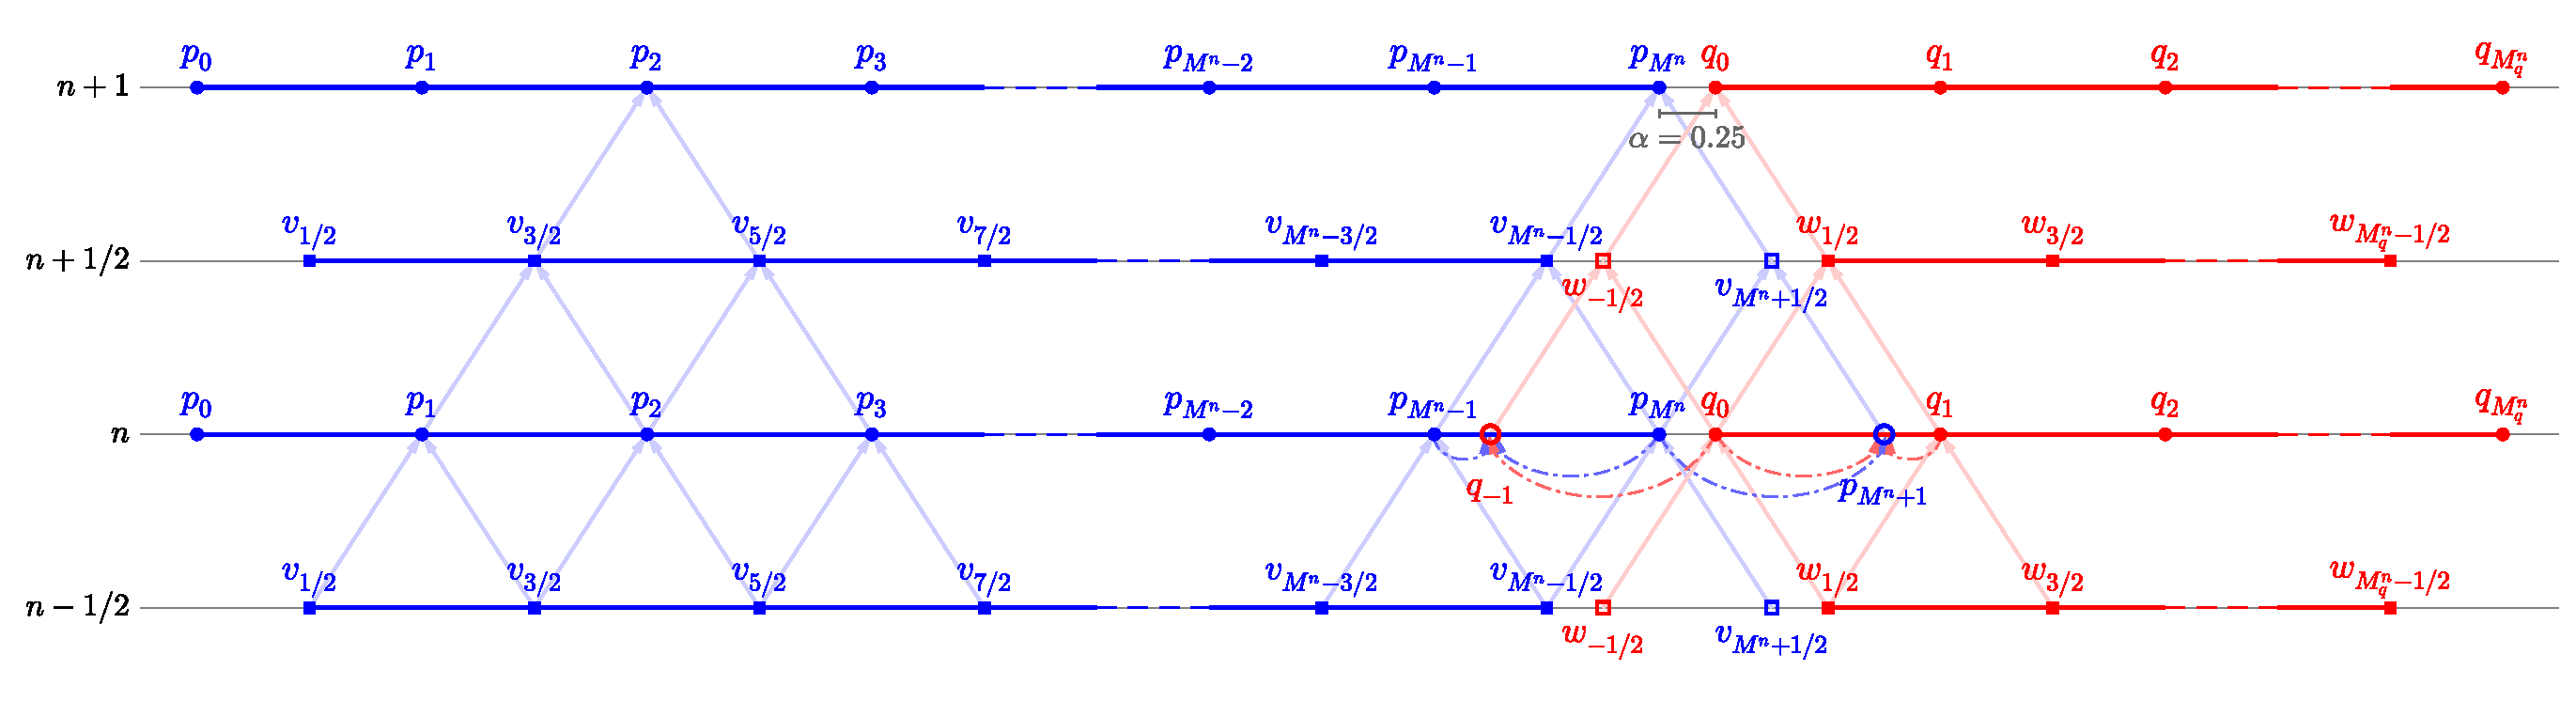
\includegraphics[width = \textwidth]{figures/tromboneSchematic.eps}
    \caption{\it Schematic showing data flow of how different grid points at time index $n+1$ are calculated with $\alpha = 0.25$ in Eq. \eqref{eq:alphaDef}. To prevent cluttering, arrows going straight up (indicating that the state of a grid point at time step $n$ is needed to calculate the state of that grid point at $n+1$) are suppressed. As an example of the usual case (refer to Eq. \eqref{eq:updateNormal}), the points required to calculate $p_2^{n+1}$ are shown. Furthermore, the points needed to calculate $p_{M^n}^{n+1}$ and $q_0^{n+1}$ are shown. The most important difference with the usual case is that the virtual grid points $p_{M^n+1}^n$ and $q_{-1}^n$ 
    are the result of the interpolation of known pressure values at $n$ using Eq. \eqref{eq:connectionInterpol}. %and velocity values at $n+1/2$ respectively
    %
    %\SWcomment[Seemingly, $q_0^n$ is not calculated from anything, but it is simply $q_0^{n+1}$ time-shifted back. The same would be shown for $v_{M_p+1/2}^{n-1/2}$, but the figure does not go back-in-time more than this.]
    \label{fig:dynamicGridSchematic}}
\end{figure*}

\section{Dynamic grid}\label{sec:dynamicGrid}
The defining feature of the trombone is its slide that alters the length of the tube, changing the resonant frequencies. In a companion paper \cite{Willemsen2021}, we present a method to dynamically change grid configurations of FD schemes by inserting and deleting grid points based on an instantaneous value of the time-varying wave speed $c(t)$. Although here, the tube length $L(t)$ is varied, the method still applies. %\SWcomment[So that's the thing. We're changing $c$ in the other paper, but $L$ here. Could change this to "an instantaneous value of the time varying wave speed $c(t)$. Although here, the tube length $L(t)$ is varied, the method still applies."] Though \cite{Willemsen2021} shows changes in the wavespeed $c$ rather than the length $L$, the effect of a change in either of these parameters has an identical effect on these systems \SWcomment[as long as the geometry is unchanged for the grid points.] Leaving $c$ fixed also means that grid spacing $h$ does not change during the simulation, but rather the spatial domain of the system. 
Note that this method only works for slow (sub-audio rate) parameter changes.
%\SBcomment[Not quite clear---in this paper, is it $c$ changing, or $L$? You might not need all this explanation of the equivalence between changing $c$ and $L$. ] \SWcomment[I'm changing $L$ so $c$ -- and $h$ -- are fixed. I just wanted to show that this method also works when changing another variable, but I guess the other paper already clarifies that.. Planning to remove "Though \cite{Willemsen2021} shows...spatial domain of the system." ]

We can split a tube with time-varying length $L^n$ into two smaller sections with lengths $L_p^n$ and $L_q^n$ (in m) such that $L^n = L_p^n + L_q^n$. Splitting the schemes in \eqref{eq:FDS} in this way yields two sets of first-order systems. The pressure and particle velocity of the first (left) system $p_\lp^n$ and $v_{\lp+1/2}^{n+1/2}$ are both defined over discrete domain $\lp \in \{0, \hdots, M^n\}$% \SBcomment[OK, here, don't totally get this...I would think $p$ would be defined over one more grid point than $v$, not over the same domains. This would be true for both the left hand domain and the right hand domain, assuming that $p$ lies at the subdomain endpoint.] \SWcomment[Alright, this is exactly what confused me too during this process, so let me try to explain (refer to Figure \ref{fig:dynamicGridSchematic} so it's easier to follow).. In order to calculate the inner boundaries at $n+1$ ($p_M^{n+1}$ and $q_0^{n+1}$) we need two (quadratically) interpolated points for the pressure at time-step $n$ ($p_{M+1}^n$ and $q_{-1}^n$). This is the method from \cite{Willemsen2021}. These interpolated points are used to calculate two "virtual" grid points for velocity at $n+1/2$ ($v_{M+1/2}^{n+1/2}$ and $w_{-1/2}^{n+1/2}$), which, in turn, are used to calculate $p_M^{n+1}$ and $q_0^{n+1}$. These two "virtual" velocity points I added to the discrete domains. This results in the ranges for $v$ and $w$ to be the same length as the pressure ranges $p$ and $q$. I started out by leaving them out (so $v_{\lp+1/2}^{n+1/2}$ for $\lp \in \{0, \hdots, M-1\}$ and $w_{\lq-1/2}^{n+1/2}$ for $\lq \in \{1,\hdots, M_q\}$) but for ease of working with the vectors later on it made more sense to include these in the ranges. Also we need to use the virtual velocities at $n-1/2$ ($v_{M+1/2}^{n-1/2}$ and $w_{-1/2}^{n-1/2}$) to eventually calculate $p_M^{n+1}$ and $q_0^{n+1}$ so also because of this, it made more sense to include them.] \SBcomment[Also, should $M$ be $M_{p}$ here?] \SWcomment[I left subscript $p$ out for brevity (like in the other paper there is no subscript $u$ for $M$ of the left system) as I'll use the $M$ as an index a lot later on.]
, and those of the second (right) system $q_\lq^n$ and $w_{\lq-1/2}^{n+1/2}$ are defined over discrete domain $\lq \in \{0, \hdots, M_q^n\}$, with
\begin{equation}\label{eq:MMq}
    M^n = \lceil L_p^n/h\rceil, \quad \text{and} \quad M_q^n = \lfloor L_q^n/h\rfloor
\end{equation} where $\lceil \cdot \rceil$ denotes the ceiling operation. Note, that the domains for $v$ and $w$ have an extra grid point when compared to the regular case in \eqref{eq:FDS} and that $w$ is indexed with $\lq-1/2$ rather than $\lq+1/2$. The resulting system of FD schemes then becomes
\begin{subequations}\label{eq:firstOrderPairs}
    \begin{align}
        \frac{\bar S_\lg}{\rho_0 c^2}\delta_{t+}p_\lp^n &= -\delta_{x-}(S_{\lg+1/2}v_{\lp+1/2}^{n+1/2}),\label{eq:discPressureP}\\
        \rho_0 \delta_{t-}v_{\lp+1/2}^{n+1/2}&=-\delta_{x+}p_\lp^n,\label{eq:discVelocityV}\\
        \frac{\bar S_\lg}{\rho_0 c^2}\delta_{t+}q_\lq^n &= -\delta_{x+}(S_{\lg-1/2}w_{\lq-1/2}^{n+1/2}),\label{eq:discPressureQ}\\
        \rho_0 \delta_{t-}w_{\lq-1/2}^{n+1/2}&=-\delta_{x-}q_\lq^n.\label{eq:discVelocityW}
    \end{align}
\end{subequations}
Here, due to the different indexing for $w$, the spatial derivatives for the right system are flipped ($\delta_{x+}$ became $\delta_{x-}$ and vice versa). Also note, that $l$ is still used for the spatial indices of $\bar S$ and $S$ which now approximate $S(x)$ according to
\begin{equation}
S_l \approx \begin{cases}
     S(x=lh) & \text{for } x\in [0, L_p^n],\\
     S(x=L^n-(M_q^n-l)h) & \text{for } x\in [L_p^n, L^n].
\end{cases}
\end{equation} 
The conditions for the outer boundaries of this system, i.e., at $\lp = 0$ and $\lq = M_q^n$, are the same as for the full system. The inner boundaries, $\lp = M^n$ and $\lq = 0$ are connected according to the method described in \cite{Willemsen2021} to be explained shortly.
To be able to calculate $p_{M^n}^{n+1}$ and $q_0^{n+1}$, the domains of $v$ and $w$ have been extended at the inner boundaries to include $v_{M^n+1/2}^{n+1/2}$ and $w_{-1/2}^{n+1/2}$. These, however, require points outside of the domains of $p_\lp^n$ and $q_\lq^n$, i.e., $p_{M^n+1}^n$ and $q_{-1}^n$. In \cite{Willemsen2021} we propose to calculate these \textit{virtual grid points} based on known values of the system. Despite the fact that \cite{Willemsen2021} presents the method using a second-order system, it can still be applied here. The process of how $p_{M^n}^{n+1}$ and $q_0^{n+1}$ are calculated is visualised in in Figure \ref{fig:dynamicGridSchematic}. Notice that all time steps use the same value of $M^n$ and $M_q^n$. In other words, the expansion of the temporal operators in \eqref{eq:discTimeOperators} do not affect the temporal indices $n$ in $M^n$ and $M_q^n$.

\subsection{Changing the Tube Length}
In the following, the location of a grid point $u_l$ along the grid (in m from the left boundary) at time index $n$ is denoted as $x_{u_l}^n$.

The two pairs of first order systems in \eqref{eq:firstOrderPairs} are placed on the same domain $x$ with
\begin{equation}\label{eq:gridLocations}
    x_{p_\lp}^n = \lp h, \quad \text{and}\quad
    x_{q_\lq}^n = L^n-(M_q^n - \lq)h,
\end{equation}
describing the locations of the left system and right system respectively. Here, it can be observed that as the tube length $L^n$ changes, the locations of the grid points of the right system will change. More specifically, as the trombone-slide is extended and $L^n$ increases, all grid points of the right system move to the right, and to the left for a contracting slide. If $L^n$ is changed in a smooth fashion, the continuous domain $x \in [0,L^n]$ will not necessarily be subdivided into an integer amount of intervals $N^n$ (of size $h = ck$). This is where a \textit{fractional} number of intervals is introduced and is defined as 
\begin{equation}\label{eq:nfrac}
    \Nfrac^n = L^n/h,
\end{equation}
which is essentially the calculation of $N$ in Eq. \eqref{eq:orderOfCalcGrid} without the flooring operation, and $N^n = \lfloor \Nfrac^n \rfloor$. The fractional part of $\Nfrac^n$ can then be calculated using
\begin{equation}\label{eq:alphaDef}
    \alpha = \alpha^n = \Nfrac^n - N^n,
\end{equation}
which describes the distance between the inner boundaries along the grid in terms of how many times $h$ would fit in-between (which is always less than once). If $\Nfrac^n = N^n$ and $\alpha = 0$, the inner boundary locations perfectly overlap, and $x_{p_{M^n}}^n = x_{q_0}^n$. This also means that the domain $x$ can be exactly divided into $N^n$ equal intervals of size $h = ck$. As the virtual grid points $p_{M^n+1}^n$ and $q_{-1}^n$ perfectly overlap with $q_{1}^n$ and $p_{M^n-1}^n$ respectively, these values can be used directly to calculate the grid points at the inner boundaries. This situation effectively acts as a rigid connection between the grid points at the inner boundaries defined as
\begin{equation}\label{eq:rigidConn}
    p_{M^n}^n = q_0^n, \quad \text{if} \ \  \alpha = 0.
\end{equation}
%
If $\alpha \neq 0$, some other definition for $p_{{M^n}+1}^n$ and $q_{-1}^n$ needs to be found. We use quadratic Lagrangian interpolation according to
\begin{subequations}\label{eq:connectionInterpol}
\begin{align}
        &p_{M^n+1}^n = \frac{\alpha - 1}{\alpha + 1}p_{M^n}^n + q_0^n - \frac{\alpha - 1}{\alpha + 1}q_1^n,
    \label{eq:calcPMp1}\\
        &q_{-1}^n
        =-\frac{\alpha - 1}{\alpha + 1}p_{M^n-1}^n + p_{M^n}^n+ \frac{\alpha - 1}{\alpha + 1}q_{0}^n\label{eq:calcQm1},
\end{align}
\end{subequations}
which can then be used to calculate $v_{M^n+1/2}^{n+1/2}$ and $w_{-1/2}^{n+1/2}$ and consequently $p_{M^n}^{n+1}$ and $q_0^{n+1}$ (see Figure \ref{fig:dynamicGridSchematic}). This process is repeated every sample. It can be shown through the rigid connection in \eqref{eq:rigidConn}, that if $\alpha=0$, the definitions in \eqref{eq:connectionInterpol} reduce to $p_{M^n+1}^n = q_1^n$ and $q_{-1}^n = p_{M^n-1}^n$ as stated before.

\subsection{Adding and removing grid points}\label{sec:addRemove}
As the tube length $L^n$ changes, $L_p^n$ and $L_q^n$ also change according to
\begin{equation}
    L_p^n = L_p^{n-1} + 0.5 L_\text{diff}^n, \quad L_q^n =  L_q^{n-1} + 0.5L_\text{diff}^n,\label{eq:updateLs} 
\end{equation}
where
\begin{equation}
    L_\text{diff}^n = L^n-L^{n-1},\label{eq:lDiff}
\end{equation}
which causes the number of intervals between grid points $M^n$ and $M_q^n$ to change as well, according to Eq. \eqref{eq:MMq}.

The following state vectors are introduced for the pressure, defined for $n+1$ and $n$ %\SWcomment[($n-1$ is used later on for the state correction, say something about that here or leave for Section \ref{sec:impStateCorr}..?)]
\begin{equation}
    \mathbf{p}^n = [p_0^n, p_1^n, ..., p_{M^n}^n]^T,\ \mathbf{q}^n = [q_0^n, q_1^n, ..., q_{M_q^n}^n]^T,
\end{equation}
and for the velocity, defined for $n+1/2$ and $n-1/2$
\begin{equation}
    \begin{aligned}
        \mathbf{v}^{n-1/2} &=  [v_{1/2}^{n-1/2}, v_{3/2}^{n-1/2}, ..., v_{M^n+1/2}^{n-1/2}]^T,\\
        \mathbf{w}^{n-1/2} &=  [w_{-1/2}^{n-1/2}, w_{1/2}^{n-1/2}, ..., w_{M_q^n-1/2}^{n-1/2}]^T,
    \end{aligned}
\end{equation}
and contain the different states over the discrete domains defined at the beginning of this section. Here, $T$ denotes the transpose operation.

If $N^n>N^{n-1}$, points are added to the left and right system in an alternating fashion: %\SWcomment[(same here for $n-1$ in the state correction, say something about that here or leave for Section \ref{sec:impStateCorr}..?)]
\begin{equation}\label{eq:addingPoint}
    \begin{aligned}
        \!\!\!\!\!&\begin{cases}
            \mathbf{p}^n = [(\mathbf{p}^n)^T, I_3\mathbf{r}^n]^T\\
            \mathbf{v}^{n-1/2} = [(\mathbf{v}^{n-1/2})^T, I_3\mathbf{z}_v^{n-1/2}]^T
        \end{cases}
        \quad\!\text{if $N^n $ is odd},\\
        \!\!\!\!\!&\begin{cases}
            \mathbf{q}^n = [I_3^\flip\mathbf{r}^n, (\mathbf{q}^n)^T]^T\\
            \mathbf{w}^{n-1/2} = [ I_3^\flip\mathbf{z}_w^{n-1/2},(\mathbf{w}^{n-1/2})^T]^T
        \end{cases}\text{if $ N^n$ is even},
    \end{aligned}
\end{equation}
where
\begin{equation}\label{eq:interpVecs}
    \begin{aligned}
        \!\!\!\!\mathbf{r}^n &= [p_{M^n-1}^n, p_{M^n}^n, q_0^n, q_1^n]^T,\\
        \!\!\!\!\mathbf{z}_v^{n-1/2} &= [v_{M^n-1/2}^{n-1/2}, v_{M^n+1/2}^{n-1/2}, w_{1/2}^{n-1/2}, w_{3/2}^{n-1/2}]^T - \boldsymbol{\eta},\\
        \!\!\!\!\mathbf{z}_w^{n-1/2} &= [v_{M^n-3/2}^{n-1/2}, v_{M^n-1/2}^{n-1/2}, w_{-1/2}^{n-1/2}, w_{1/2}^{n-1/2}]^T+ \boldsymbol{\eta}^{\flip},% \quad\text{and}\\
        %     \mathbf{v}_\star^n &= [w_1^n, w_0^n, u_M^n, u_{M-1}^n],
    \end{aligned}
\end{equation}
and cubic Lagrangian interpolator
\begin{equation}\label{eq:customIp}
    I_3 = \begin{bmatrix} -\frac{\alpha(\alpha+1)}{(\alpha+2)(\alpha+3)} &\frac{2\alpha}{\alpha+2} &\frac{2}{\alpha+2} 
    &-\frac{2\alpha}{(\alpha+3)(\alpha+2)}
    \end{bmatrix}.
\end{equation}
Here, 
\begin{equation}\label{eq:offsetVec}
    \boldsymbol{\eta} = \boldsymbol{\eta}^{n-1/2}= \left(w_{-1/2}^{n-1/2}-v_{M^n+1/2}^{n
    -1/2}\right)\cdot[0, 0, 1, 1]^T 
\end{equation}
adds an offset to half of the elements in the $\mathbf{z}$ vectors depending on the difference between $v_{M^n+1/2}^{n-1/2}$ and $w_{-1/2}^{n-1/2}$. Why this is necessary will be further explained in Section \ref{sec:drift}. Finally, $I_3^\flip$ and $\boldsymbol{\eta}^{\flip}$ are flipped versions of \eqref{eq:customIp} and \eqref{eq:offsetVec} respectively.

If $N^n < N^{n-1}$, points are simply removed from the vectors according to
\begin{equation}\label{eq:removingPoint}
    \begin{aligned}
        &\!\!\!\!\!\!\begin{cases}
            \mathbf{p}^n = [p_0^n, \hdots, p_{M^n-1}^n]^T\\
            \mathbf{v}^{n-1/2} = [v_{1/2}^{n-1/2}, \hdots, v_{M^n-1/2}^{n-1/2}]^T
        \end{cases}
        \quad\!\text{if $N^n$ is even},\\
        &\!\!\!\!\!\!\begin{cases}
            \mathbf{q}^n = [q_1^n, \hdots, q_{M_q^n}^n]^T\\
            \mathbf{w}^{n-1/2} = [w_{1/2}^{n-1/2},\hdots, w_{M_q^n-1/2}^{n-1/2}]^T
        \end{cases}\text{if $ N^n$ is odd}.
    \end{aligned}
\end{equation}
Notice that the even and odd conditions in Eqs. \eqref{eq:addingPoint} and \eqref{eq:removingPoint} can be swapped. To stay as close to the desired location of adding and  removing grid points as possible, this requires the ceiling and flooring operations in \eqref{eq:MMq} to be swapped as well.
\subsection{Drift of $w$}\label{sec:drift}
The inner boundaries of the pressure states $p$ and $q$ are connected by \eqref{eq:connectionInterpol}, but no such connection exists for the velocity states $v$ and $w$. As the radiating boundary is implemented on the pressure grid, this leaves $w$ without any boundary condition; it is only ``held in place'' by the pressure values of $q$, or more specifically, by derivatives (both spatial and temporal). As FD schemes are an approximation, it does not give a perfect solution and $w$ tends to `drift' during the simulation, especially when $L^n$ is changed.

Luckily, as the pressure values are also calculated from derivatives of the velocity, the absolute state of $w$ does not matter. The difference in values at the connection point is also irrelevant as there is no spatial derivative taken between $v$ and $w$ (refer to Figure \ref{fig:dynamicGridSchematic}). Finally, the pressure values are used for the output audio of the simulation, so the drift does not affect the audio. 

The absolute states of the velocity vectors do, however, need to be accounted for when adding points to the $\mathbf{v}$ and $\mathbf{w}$ using \eqref{eq:addingPoint}. The current drift can be approximated by observing the difference between $w_{-1/2}^{n-1/2}$ and $v_{M^n+1/2}^{n-1/2}$, as these have approximately the same $x$ location ($x_{w_{-1/2}}^n \approx x_{v_{M^n+1/2}}^n$) when a grid point is added. This is then used in a drift-correction vector $\boldsymbol{\eta}^{n-1/2}$ presented in \eqref{eq:offsetVec}. When a point is added to $v$, the values of $w$ in $\mathbf{z}_{v}$ are offset by the aforementioned difference and when a point is added to $w$ the same happens (inverted) for the values of $v$ in $\mathbf{z}_w$. This way, the drift is allowed, but does not affect the state of the newly added grid points. Notice that the drift does not affect the operations of point removal in \eqref{eq:removingPoint}.

\subsection{State Correction}
As $L^n$, and consequently the number of grid points, is decreased, it might occur that the grid points at the inner boundaries $p_{M^n}^n$ and $q_0^n$ have a very different value when $\alpha \gtrsim 0$, i.e., right before a point is removed. This violates the rigid connection in Eq. \eqref{eq:rigidConn}. 

We propose in \cite{Willemsen2021} to add an artificial spring-like connection between the grid points at the inner boundaries that ``corrects'' the state of these points. Applying this to system \eqref{eq:firstOrderPairs} extends Eqs. \eqref{eq:discPressureP} and \eqref{eq:discPressureQ} according to
\begin{subequations}\label{eq:pressuresWithSC}
    \begin{align}
        \frac{\bar S_\lg}{\rho_0 c^2}\delta_{t+}p_\lp^n &= -\delta_{x-}(S_{\lg+1/2}v_{\lp+1/2}^{n+1/2}) + J_p(x_{p_{M^n}}^n)F_\text{sc}^n,\label{eq:pWithSC}\\
        \frac{\bar S_\lg}{\rho_0 c^2}\delta_{t+}q_\lq^n &= -\delta_{x+}(S_{\lg-1/2}w_{\lq-1/2}^{n+1/2}) - J_q(x_{q_0}^n)F_\text{sc}^n,\label{eq:qWithSC}
    \end{align}
\end{subequations}
where the spreading operators are defined as
\begin{equation}\label{eq:spreadingOperators}
    \begin{aligned}
    J_p(x_i^n)& =
    \begin{cases}
        \frac{1}{h}, & \lp = \lfloor x_i^n/h\rfloor\\
        0,& \text{otherwise},
    \end{cases}
    \quad\text{and}\\
    J_q(x_i^n) &=
    \begin{cases}
        \frac{1}{h}, & \lq = \lfloor x_i^n/h \rfloor - M^n\\
        0,& \text{otherwise}.
    \end{cases}
\end{aligned}
\end{equation}
Furthermore, the correction effect is defined as
\begin{equation}\label{eq:scForce}
    F_\text{sc}^n = \beta\left(\mu_{t\cdot}\eta_\text{sc}^n+\sigma_\text{sc}\delta_{t\cdot}\eta_\text{sc}^n\right),
\end{equation}
% (in m$^{3}$/s)\SWcomment[..units stop making sense here as this is an artificial connection ``force''.. might just exclude them?]
with spring damping $\sigma_\text{sc}$, pressure difference
\begin{equation}
    \eta_\text{sc}^n \triangleq q_0^n - p_{M^n}^n,
\end{equation} 
and scaling coefficient
\begin{equation}\label{eq:betaDef}
    \beta = \beta(\alpha) = \frac{1-\alpha}{\alpha+\varepsilon}.
\end{equation}
Here, $\varepsilon\ll 1$ to prevent division by 0. Just like in \cite{Willemsen2021}, the implementation of the correction effect allows for an infinite $\beta$ when $\alpha = \varepsilon = 0$ acting like a rigid connection between Eqs. \eqref{eq:pWithSC} and \eqref{eq:qWithSC}.
% One can write the entire system above in matrix form by concatenating...

\begin{table}[t]
    \small
    \begin{center}
    \caption{\it Geometry of a measured trombone taken from \cite{Smyth2011}. Numbers correspond to Figure \ref{fig:tromboneSchematic}.\label{tab:geometry}}
    \begin{tabular}{|l|c|c|}
        \hline
        Part of tube & Length (cm) & Radius (cm)\\\hline
        Inner slide (1) & 70.8 & 0.69\\
        Outer slide (extended) (2) & 53 & 0.72 
        \\
        Slide crook (3)& 17.7 & 0.74\\
        Outer slide (extended) (4) & 53 & 0.72 
        \\
        Inner slide (5) & 71.1 & 0.69\\
        Gooseneck (6) & 24.1 & 0.71\\
        Tuning slide (7) & 25.4 & 0.75, 1.07\\
        Bell flare (8) & 50.2& 1, 10.8\\\hline
    \end{tabular}
    \end{center}
\end{table}

\begin{table}[t]
    \small
    \begin{center}
    \caption{\it List of parameter values used for the simulation. 
    Taken from $^\star$\cite{Smyth2011}, *\cite{Harrison2018} or **\cite{Benade1968} with temperature $T=26.85^\circ C$. \label{tab:parameters}}
    \begin{tabular}{|l|c|c|}
        \hline
        Name & Symbol (unit) & Value\\ \hline
        \multicolumn{3}{|l|}{\bf Tube}\\ \hline
        Length & $L$ (m) & $2.593\leq L \leq 3.653$$^\star$\\
        Air density &$\rho_0$ (kg/m$^3$) & 1.1769** 
        \\
        Wave speed & $c$ (m/s) & 347.23**\\
        Geometry & $S$ (m$^2$) & See Table \ref{tab:geometry}. \\\hline
        \multicolumn{3}{|l|}{\bf Lip reed}\\ \hline
        Mass & $M_\text{r}$ (kg) & $5.37\cdot10^{-5}$*\\
        Frequency & $\omega_\text{r}$ (rad/s) & $ 20\leq \omega_\text{r}/2\pi \leq 1000$\\
        Mouth pressure & $P_\text{m}$ (Pa) & $0 \leq P_\text{m} \leq 6000$\\
        Damping & $\sigma_\text{r}$ (s$^{-1}$) & $5$*\\
        Eff. surface area & $S_\text{r}$ (m$^{2}$) & $1.46\cdot 10^{-5}$*\\
        Width & $w_\text{r}$ (m) & $0.01$* \\
        Equilibrium sep. & $H_0$ (m) &  $2.9 \cdot 10^{-4}$* \\
        Coll. stiffness& $K_\text{c}$ (N/m) & $10^4$\\
        Nonlin. coll. coeff.& $\alpha_\text{c}$ (-)  &3\\\hline
        \multicolumn{3}{|l|}{\bf Other}\\ \hline
        % State corr. stiffness & $\omega_\text{sc}$ & $1$\\ 
        State corr. damping & $\sigma_\text{sc}$ & $1$\\ 
        Sample rate & $f_\text{s}$ (Hz) & 44100\\
        \hline
    \end{tabular}
    \end{center}
\end{table}
\begin{figure}[t]
    \centering
    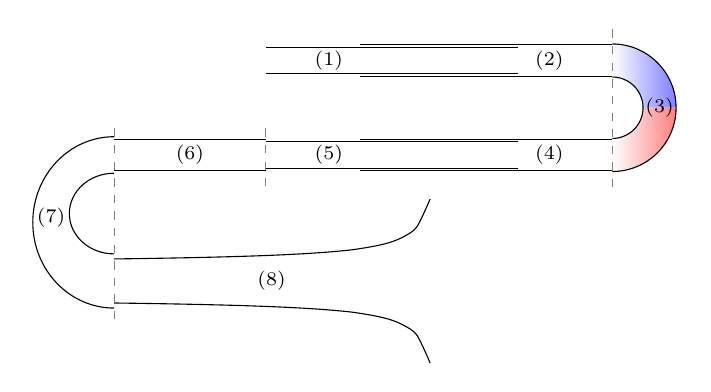
\begin{tikzpicture}[scale = 8]

    \def\labelColor{black};
    \def\labelSize{\fontsize{7pt}{7pt}\selectfont};

    \def\hornOffset{0.025};
    \def\stepSize{0.004}

    \def\dashedLineColor{gray};
    \def\dashedLineOvershoot{0.025}
    % tuning slide params
    \def\tuningSlideDim{0.1};
    \pgfmathsetmacro{\tuningSlideRad}{\stepSize + \hornOffset};
    \def\tuningSlideOffset{0.007};

    % gooseneck params
    \def\gooseNeckLength{0.241};
    \pgfmathsetmacro{\gooseNeckRad}{\tuningSlideRad - \stepSize};

    % inner slide params
    \def\innerLength{0.4};
    \pgfmathsetmacro{\innerRad}{\gooseNeckRad - \stepSize};

    % outer slide params
    \def\outerLength{\innerLength};
    \pgfmathsetmacro{\outerRad}{\gooseNeckRad};
    \pgfmathsetmacro{\extension}{0.15};

    \def\endOfSlideDim{0.075};
    \pgfmathsetmacro{\endOfSlideRad}{\outerRad * 1.05};

    %% draw horn

    \draw[domain=0:0.502, smooth, variable=\x, black] plot ({\x}, {\hornOffset + 0.0063 * ((0.502-\x) + 0.0174)^(-0.7)});
    
    \draw[domain=0:0.502, smooth, variable=\x, black] plot ({\x}, {-\hornOffset-0.0063 * ((0.502-\x) + 0.0174)^(-0.7)});
    
    \node[anchor = center, color = \labelColor](eight) at (0.25, 0) {\labelSize(8)};

    % draw tuningSlide
    \pgfmathsetmacro{\innerTuningSlideDim}{(\tuningSlideDim - \tuningSlideRad)}
    \pgfmathsetmacro{\outerTuningSlideDim}{(\tuningSlideDim + \tuningSlideRad)}

    \node[anchor = center, color = \labelColor](seven) at (-\innerTuningSlideDim-\tuningSlideRad, \innerTuningSlideDim+\tuningSlideRad) {\labelSize(7)};

    \pgfmathsetmacro{\innerTuningSlideWithOffset}{\innerTuningSlideDim - \tuningSlideOffset}

    \pgfmathsetmacro{\outerTuningSlideWithOffset}{\outerTuningSlideDim + \tuningSlideOffset}

    \draw (0, 2*\tuningSlideDim-\tuningSlideRad) arc(90:270:\innerTuningSlideDim cm and \innerTuningSlideWithOffset cm);

    \draw (0, 2*\tuningSlideDim+\tuningSlideRad) arc(90:270:\outerTuningSlideDim cm and \outerTuningSlideWithOffset cm);
    
    % dashedline
    \draw[dashed, color = \dashedLineColor] (0, -\tuningSlideRad-\tuningSlideOffset-\dashedLineOvershoot) -- (0, 2*\tuningSlideDim+\tuningSlideRad+\dashedLineOvershoot);

    % draw gooseneck
    \draw (0, 2*\tuningSlideDim + \gooseNeckRad) -- (\gooseNeckLength, 2*\tuningSlideDim + \gooseNeckRad);

    \draw (0, 2*\tuningSlideDim - \gooseNeckRad) -- (\gooseNeckLength, 2*\tuningSlideDim - \gooseNeckRad);

    \node[anchor = center, color = \labelColor](six) at (0.5 * \gooseNeckLength, 2*\tuningSlideDim) {\labelSize(6)};

    % dashedline
    \draw[dashed, color = \dashedLineColor] (\gooseNeckLength, 2*\tuningSlideDim-\gooseNeckRad-\dashedLineOvershoot) -- (\gooseNeckLength, 2*\tuningSlideDim+\gooseNeckRad+\dashedLineOvershoot);

    % draw inner slide
    \draw (\gooseNeckLength, 2*\tuningSlideDim + \innerRad) -- (\gooseNeckLength+\innerLength, 2*\tuningSlideDim + \innerRad);

    \draw (\gooseNeckLength, 2*\tuningSlideDim - \innerRad) -- (\gooseNeckLength+\innerLength, 2*\tuningSlideDim - \innerRad);

    \node[anchor = center, color = \labelColor](five) at (\gooseNeckLength + 0.25 * \innerLength, 2*\tuningSlideDim) {\labelSize(5)};

    % draw outer slide
    \pgfmathsetmacro{\outerSlideStart}{\gooseNeckLength + \extension};

    \draw (\outerSlideStart, 2*\tuningSlideDim + \outerRad) -- (\outerSlideStart+\outerLength, 2*\tuningSlideDim + \outerRad);

    \draw (\outerSlideStart, 2*\tuningSlideDim - \outerRad) -- (\outerSlideStart+\outerLength, 2*\tuningSlideDim - \outerRad);

    \node[anchor = center, color = \labelColor](four) at (\outerSlideStart + 0.75 * \outerLength, 2*\tuningSlideDim) {\labelSize(4)};


    % draw end of slide
    
    \pgfmathsetmacro{\innerEndOfSlideDim}{(\endOfSlideDim - \endOfSlideRad)};
    \pgfmathsetmacro{\outerEndOfSlideDim}{(\endOfSlideDim + \endOfSlideRad)};

    \pgfmathsetmacro{\startEndOfSlide}{\outerSlideStart + \outerLength};
    % division blue
    \fill[white, left color=white, right color=blue, fill opacity = 0.5] 
    (\startEndOfSlide+\innerEndOfSlideDim,2*\tuningSlideDim+\endOfSlideDim) 
    arc (0:90:\innerEndOfSlideDim cm and \innerEndOfSlideDim cm) 
    -- (\startEndOfSlide,2*\tuningSlideDim+\endOfSlideDim + \innerEndOfSlideDim)
    -- (\startEndOfSlide,2*\tuningSlideDim+2*\endOfSlideDim+\endOfSlideRad)
    arc (90:0:\outerEndOfSlideDim cm and \outerEndOfSlideDim cm)
    -- (\startEndOfSlide+\outerEndOfSlideDim,2*\tuningSlideDim+\endOfSlideDim)
    -- cycle;

    % division red
    \fill[white, left color=white, right color=red, fill opacity = 0.5] 
    (\startEndOfSlide+\innerEndOfSlideDim,2*\tuningSlideDim+\endOfSlideDim) 
    arc (0:-90:\innerEndOfSlideDim cm and \innerEndOfSlideDim cm) 
    -- (\startEndOfSlide,2*\tuningSlideDim+\endOfSlideDim)
    -- (\startEndOfSlide,2*\tuningSlideDim-\endOfSlideRad)
    arc (-90:0:\outerEndOfSlideDim cm and \outerEndOfSlideDim cm)
    -- (\startEndOfSlide+\outerEndOfSlideDim,2*\tuningSlideDim+\endOfSlideDim)
    -- cycle;

    \draw (\startEndOfSlide, 2*\tuningSlideDim+\endOfSlideRad) arc(-90:90:\innerEndOfSlideDim cm and \innerEndOfSlideDim cm);

    \draw (\startEndOfSlide, 2*\tuningSlideDim-\endOfSlideRad) arc(-90:90:\outerEndOfSlideDim cm and \outerEndOfSlideDim cm);

    \node[anchor = center, color = \labelColor](three) at (\startEndOfSlide + \innerEndOfSlideDim + \endOfSlideRad, 2*\tuningSlideDim+ \innerEndOfSlideDim + \endOfSlideRad) {\labelSize(3)};


    % dashedline
    \draw[dashed, color = \dashedLineColor] (\startEndOfSlide, 2*\tuningSlideDim-\endOfSlideRad-\dashedLineOvershoot) -- (\startEndOfSlide, 2*\tuningSlideDim+2*\endOfSlideDim+\endOfSlideRad+\dashedLineOvershoot);

    % draw second outer slide

    \draw (\outerSlideStart, 2*\tuningSlideDim + 2 * \endOfSlideDim + \outerRad) -- (\outerSlideStart+\outerLength, 2*\tuningSlideDim + 2 * \endOfSlideDim + \outerRad);

    \draw (\outerSlideStart, 2*\tuningSlideDim + 2 * \endOfSlideDim - \outerRad) -- (\outerSlideStart+\outerLength, 2*\tuningSlideDim + 2 * \endOfSlideDim - \outerRad);

    \node[anchor = center, color = \labelColor](two) at (\outerSlideStart + 0.75 * \outerLength, 2*\tuningSlideDim + 2 * \endOfSlideDim) {\labelSize(2)};

    % draw inner slide
    \draw (\gooseNeckLength, 2*\tuningSlideDim+ 2 * \endOfSlideDim + \innerRad) -- (\gooseNeckLength+\innerLength, 2*\tuningSlideDim+ 2 * \endOfSlideDim + \innerRad);

    \draw (\gooseNeckLength, 2*\tuningSlideDim + 2 * \endOfSlideDim - \innerRad) -- (\gooseNeckLength+\innerLength, 2*\tuningSlideDim + 2 * \endOfSlideDim - \innerRad);

    \node[anchor = center, color = \labelColor](one) at (\gooseNeckLength + 0.25 * \innerLength, 2*\tuningSlideDim + 2 * \endOfSlideDim) {\labelSize(1)};

% \begin{scope}[very thick,decoration={
%     markings,
%     mark=at position 0.5 with {\arrow{>}}}
%     ] 
%     \draw[postaction={decorate}] (-4,0)--(4,0);
% \end{scope}
    
    \end{tikzpicture}
    \caption{\it Diagram showing the trombone geometry (not to scale). Numbers correspond to the parts of the tube found in Table \ref{tab:geometry} and dashed lines highlight where the different parts are separated. The tube is split in the middle of the slide crook with the colours corresponding to those in Figure \ref{fig:dynamicGridSchematic}.}
    \label{fig:tromboneSchematic}
\end{figure}
\vspace{-1em}
\section{Implementation}\label{sec:implementation}
The implementation has been done in C++ using the JUCE framework \footnote{\href{https://juce.com/}{https://juce.com/}}, and is available online\footnote{\href{https://github.com/SilvinWillemsen/cppBrass/releases/}{https://github.com/SilvinWillemsen/cppBrass/releases/}} as well as a demo showcasing it.\footnote{\href{https://youtu.be/Ht5gVNrshYo}{https://youtu.be/Ht5gVNrshYo}} The audio output of the system can be retrieved by selecting a grid point on the pressure grid and listening to this at the given sample rate $f_\text{s}$. Here, the radiating boundary $q_{M_q^n}^n$ is chosen, as this is where the sound enters the listening space in the real world. %the output is taken as the weighted average of the rightmost points until 10.8 cm (radius of the flare-end) from the end of the the radiating boundary. This range was chosen due to the fact that in the real world, the sound does not originate from a single point-like source, but rather from a larger -- here assumed to be spherical -- region of space. The spatial averaging has a low-passing effect on the sound, but informal listening tests by the authors have confirmed that the sound is more true to that of an actual trombone than if a single point is chosen. 
To mimic low-pass filtering happening due to a distributed radiating area, a 4\textsuperscript{th}-order low-passing Butterworth filter with a cutoff frequency of $f_\text{c}= \sqrt{c^2\pi/S(L)} \approx 3245$ Hz is used. This equation is retrieved by choosing the listening point to be at the bell surface and integrating over the bell area. 

% We continue by providing the parameter values used in the simulation.
\subsection{Parameters}
For the most part, the parameters used in the simulation have been obtained from \cite{Harrison2018, Smyth2011, Benade1968}. The lengths and radii of different parts of the tube can be found in Table \ref{tab:geometry} and a diagram showing this geometry is shown in Figure \ref{fig:tromboneSchematic}.
The system is split in the middle of the slide crook such that the ranges for the lengths of the two tubes are $L_p^n \in[0.797, 1.327]$ and $L_q^n \in [1.796, 2.326]$.

Other parameters used in the simulation can be found in Table \ref{tab:parameters}. Not included here is $\lambda$, which has been set slightly lower than the stability condition in \eqref{eq:CFL}, i.e., $\lambda = 0.999$. Although the implementation works when $\lambda = 1$, this is done to tolerate (much) higher speeds of change in $L^n$ before instability occurs (see Section \ref{sec:limit}). Not satisfying condition \eqref{eq:CFL} causes bandlimiting and dispersive effects \cite{bilbao2009}, but such a small deviation from the condition has no perceptual influence on the output sound and outweighs the problems caused by instability.

As the tube acts mainly as an amplifier for specific resonant frequencies it is important to match the frequency of the lip reed to a resonating mode of the tube. This frequency depends on $L^n$ in the following way
\begin{equation}\label{eq:lipReedCalc}
    \omega_\text{r}^{n+1/2} = \mathcal{F}\frac{2\pi c}{\rho_0 L^{n+1/2}}\ ,
\end{equation}
where $L^{n+1/2} = L^n$ and scalar multiplier $\mathcal{F} = 2.4$ was heuristically found to best match the 4\textsuperscript{th} resonating mode of the tube and generates a recognisable brass sound.

\subsection{Limit on speed of change}\label{sec:limit}
To reduce audible artifacts and instability issues from adding and removing points, and to stay in the sub-audio rate regime, a limit can be placed on \eqref{eq:lDiff} as
\begin{equation}\label{eq:Nmaxdiff} 
    L_\text{diff}^n \leq \Nfrac_\text{maxdiff} h,
\end{equation}
where $\Nfrac_\text{maxdiff}$ is the maximum change in $\Nfrac$ per sample and has been set to $\Nfrac_\text{maxdiff} = 1/20$. This means that a grid point can be added or removed every 20 samples and allows the entire range of $L$ to be traversed in ca. 0.06 s at a sample rate of $f_\text{s} = 44100$ Hz.

\subsection{State correction}\label{sec:impStateCorr}
The introduction of system states at $n+1$ through the centred operators in Eq. \eqref{eq:scForce} seem to make the scheme implicit. It is, however, possible to calculate $F_\text{sc}$ explicitly \cite{bilbao2009, bilbao2009dafx}. The same operators also introduce the need for values at $n-1$, i.e., $p_{M^n}^{n-1}$ and $q_{0}^{n-1}$. Therefore, the vectors $\mathbf{p}^{n-1}$ and $\mathbf{q}^{n-1}$ will need to be stored, and the operations to add and remove grid points as described in \ref{sec:addRemove} need to be applied to these as well. One could argue that only two points at the inner boundaries are needed for the calculation and to create $\mathbf{r}$ in \eqref{eq:interpVecs} at $n-1$. For generality, we continue with the entire vectors defined over the same domains as $\mathbf{p}^n$ and $\mathbf{q}^n$ respectively. 
\begin{figure}[t]
    \centering
    \setlength{\fboxsep}{0pt} 
    \fbox{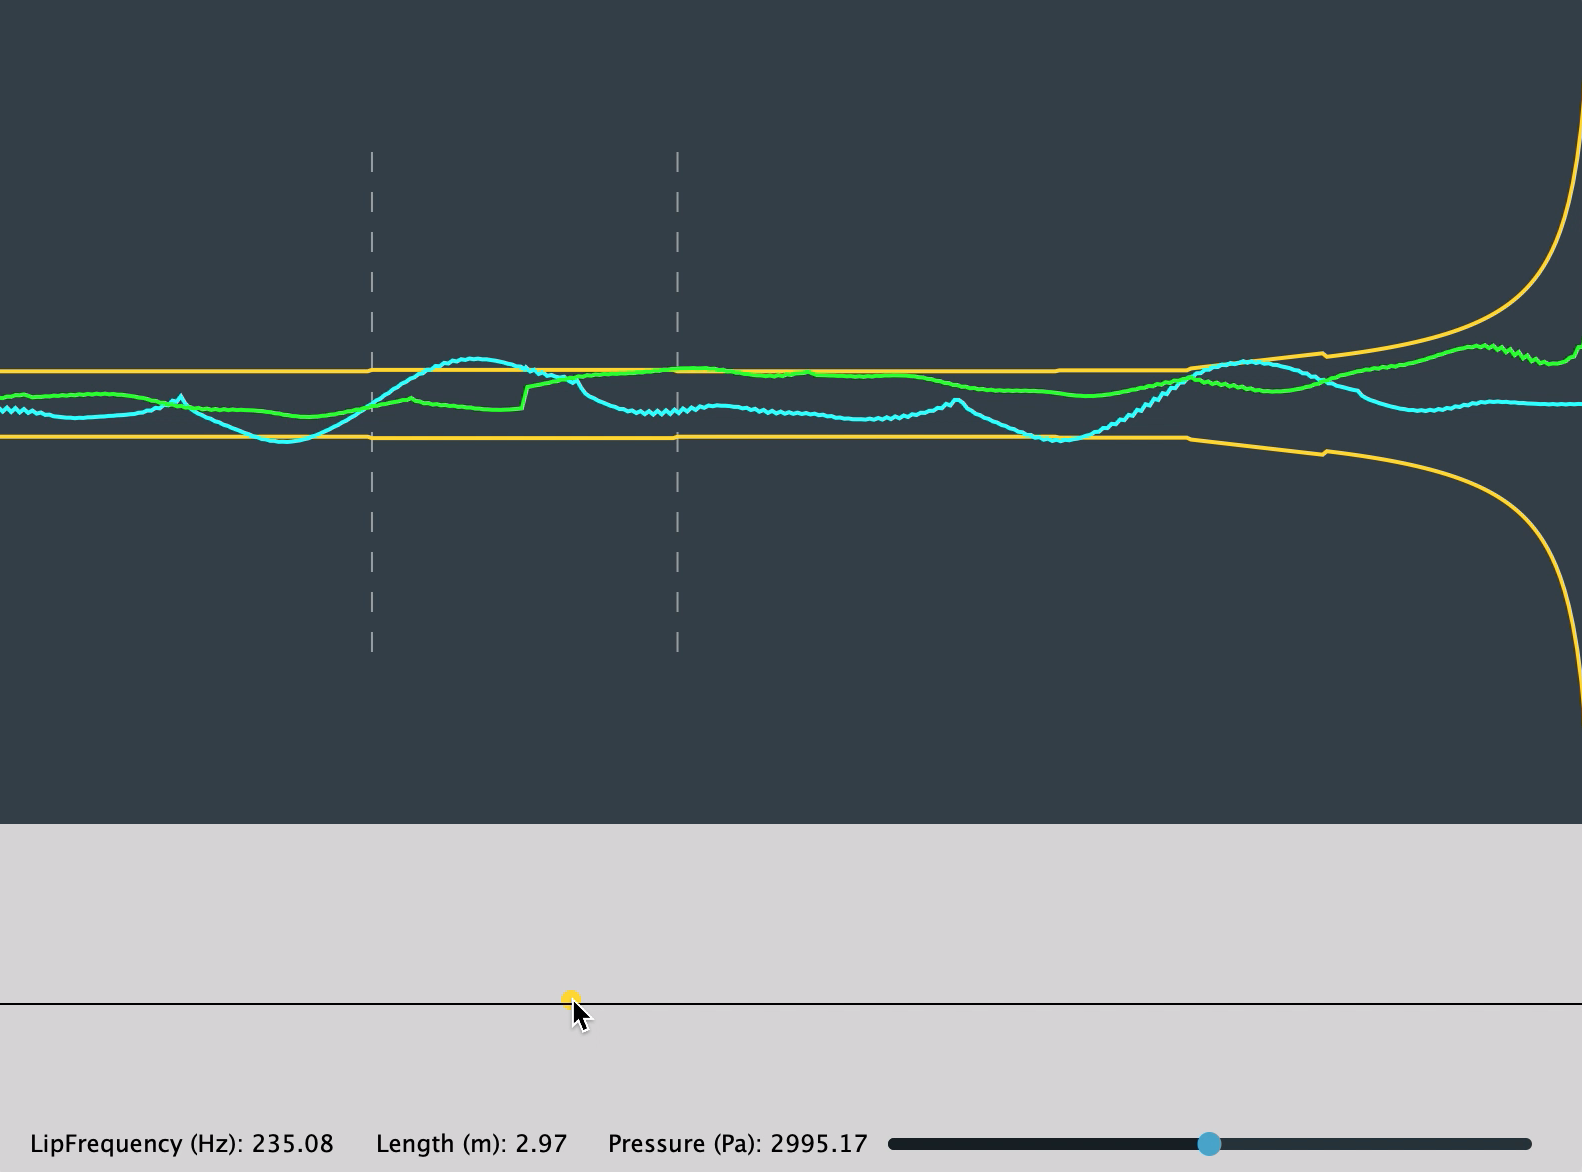
\includegraphics[width = \paperFigWidth\textwidth]{figures/GUI.png}}
    \caption{\it Screenshot of the graphical user interface (GUI). The geometry (in orange) as well as the states of the pressure (in blue) and velocity scaled by $S$ (in green) are shown. For clarity, the start and end of the outer slide are denoted by dashed lines. The drift of $w$ as explained in Section \ref{sec:drift} is visible from the ``kink'' in the green line exactly in the middle of the outer slide.}
    \label{fig:GUI}
\end{figure}

\subsection{Graphical User Interface and Control Mapping}
A screenshot of the graphical user interface (GUI) is shown in Figure \ref{fig:GUI}. The geometry of the tube is plotted along with paths showing the pressure states in blue and the velocity (scaled by the geometry $S$) in green. The audio thread of the application runs at 44100 Hz whereas the graphics are updated at a rate of 15 Hz. 

The real-time application is controlled by interacting with the bottom panel using the mouse. The x-axis is mapped to tube-length $L^n$ and also modifies the lip-reed frequency $\omega_\text{r}$ according to Eq. \eqref{eq:lipReedCalc}. The y-axis changes the multiplier $\mathcal{F}$ in Eq. \eqref{eq:lipReedCalc} and the black line in the vertical middle of the control panel is mapped to $\mathcal{F} = 2.4$. The pressure is modulated by a slider at the bottom of the control panel. As of now, no focus has been put on intuitive parameter mapping; it has only been implemented for simple parameter exploration.

% \begin{algorithm}[ht]
%     \setstretch{1.1}
%     \fbox{\parbox{0.88\linewidth}
%     {
%         \While{application is running}
%         {
%             Retrieve new parameters ($L^n$, $\omega_\text{r}^n$ and $P_\text{m}^n$) \\
%             Update $L_p^n$ and $L_q^n$ (Eqs. \eqref{eq:lDiff}, \eqref{eq:Nmaxdiff} and \eqref{eq:updateLs})\\
%             Calc. $\Nfrac^n$ and $N^n$ (Eqs. \eqref{eq:nfrac} and \eqref{eq:numberOfIntervals}) \\
%             Calc. $\alpha$ (Eq. \eqref{eq:alphaDef})\\
%             \If{$ N^n \neq N^{n-1} $}
%             {
%                 Add or remove point (Eq. \eqref{eq:addingPoint} or \eqref{eq:removingPoint})\\
%                 Update $M$ and $M_q$ (Eq. \eqref{eq:MMq})
%             }
%             Calc. $p_{M+1}^n$ and $q_{-1}^n$ (Eqs. \eqref{eq:connectionInterpol})\\
%             Calc. $\mathbf{v}^{n+1/2}$ and  $\mathbf{w}^{n+1/2}$ (Eqs. \eqref{eq:discVelocityV} and \eqref{eq:discVelocityW})\\
%             Calc. $y^{n+3/2}$ w/o collision (Eqs. \eqref{eq:discreteLipSystem})\\
%             Calc $g^{n+1/2}$ (Eq. \eqref{eq:gDef})\\
%             Calc. $y^{n+3/2}$ with collision (Eqs. \eqref{eq:discreteLipSystem})\\
%             Calc. $U_\text{B}^{n+1/2}$ and $U_\text{r}^{n+1/2}$ (Eqs. \eqref{eq:bernoulli} and \eqref{eq:Ur})\\
%             Calc. $\mathbf{p}^{n+1}$ and $\mathbf{q}^{n+1}$ (Eqs. \eqref{eq:pressuresWithSC})\\ 
%             Retrieve output\\
%             Update system states ($\mathbf{p}^{n-1} = \mathbf{p}^{n}$, $\mathbf{p}^n=\mathbf{p}^{n+1}$)\\
%             (same for $\mathbf{v}^{n-1/2} = \hdots$, $y^{n-1/2}$, $y^{n+1/2}$, and $\psi^n$),\\
%             % \begin{minipage}[c]{0.4\linewidth} 
%             % Update system states\\
%             % \\
%             % \\
%             % \\
%             % \end{minipage} \begin{minipage}[c]{0.5\linewidth} 
%             % $\mathbf{p}^{n-1} = \mathbf{p}^n$, $\mathbf{p}^n = \mathbf{p}^{n+1}$,\\
%             % $\mathbf{v}^{n-1/2} = \mathbf{v}^{n+1/2}$,\\
%             % $y^{n-1/2} = y^{n+1/2}$,\\
%             % $y^{n+1/2} = y^{n+3/2}$, \\
%             % $\psi^{n} = 
%             % \psi^{n+1}$, 
%             % \end{minipage}\\
%             Update $N$ ($N^{n-1} = N^n$)\\
%             Increment $n$            % \begin{minipage}[c]{0.4\linewidth}
%             % -\\
%             % \vspace{2em}(Eq. \eqref{eq:addingPoint})\\
            
%             % (Eq. \eqref{eq:removingPoint})\\

%             % \end{minipage}
%             }
%         }
%     }
%     \vspace{0.12cm}
%     \caption{Pseudocode showing the order of calculations of the algorithm implementing the trombone .\label{alg:calcOrder}}
% \end{algorithm}
\begin{algorithm}[t]
    \setstretch{1.1}
    \fbox{\parbox{0.88\linewidth}
    {
        \While{application is running}
        {
            \begin{minipage}[c]{0.48\linewidth}
                Retrieve new parameters\\
                Update $L_p^n$ and $L_q^n$\\
                Calc. $\Nfrac^n$ and $N^n$\\
                Calc. $\alpha^n$ \\
                \If{$ N^n \neq N^{n-1} $}
                {
                    Add or remove point\\
                    Update $M^n$ and $M_q^n$ 
                }
                Calc. $p_{M^n+1}^n$ and $q_{-1}^n$ \\
                Calc. $\mathbf{v}^{n+1/2}$ and  $\mathbf{w}^{n+1/2}$ \\
                Calc. $y^{n+3/2}$ w/o collision \\
                Calc $g^{n+1/2}$ \\
                Calc. $y^{n+3/2}$ with collision \\
                Calc. $U_\text{B}^{n+1/2}$ and $U_\text{r}^{n+1/2}$ \\
                Calc. $\mathbf{p}^{n+1}$ and $\mathbf{q}^{n+1}$ \\
                Retrieve output
            \end{minipage}
            \begin{minipage}[c]{0.43\linewidth}
                ($L^n$, $\omega_\text{r}^n$ and $P_\text{m}^n$) \\
                (Eqs. \eqref{eq:lDiff}, \eqref{eq:Nmaxdiff} \& \eqref{eq:updateLs})\\
                (Eqs. \eqref{eq:nfrac} and \eqref{eq:orderOfCalcGrid})\\
                (Eq. \eqref{eq:alphaDef})\\
                \vspace{-0.2em}\\
                (Eq. \eqref{eq:addingPoint} or \eqref{eq:removingPoint})\\
                (Eq. \eqref{eq:MMq})\\
                \vspace{-0.15em}\\
                (Eqs. \eqref{eq:connectionInterpol})\vspace{0.05em}\\
                (Eqs. \eqref{eq:discVelocityV} and \eqref{eq:discVelocityW})\\
                (Eqs. \eqref{eq:discreteLipSystem})\\
                (Eq. \eqref{eq:gDef})\\
                (Eqs. \eqref{eq:discreteLipSystem})\\
                (Eqs. \eqref{eq:bernoulli} and \eqref{eq:Ur})\\
                (Eqs. \eqref{eq:pressuresWithSC})
                \vspace{0.25em}\\
           \end{minipage}
           \\
           \begin{minipage}[c]{0.4\linewidth}
                Update system states\\
                \\
                \\
                Update $N^{n-1}$ \\
                Increment $n$      
            \end{minipage}
            \begin{minipage}[c]{0.5\linewidth}
                ($\mathbf{p}^{n-1} = \mathbf{p}^{n}$, $\mathbf{p}^n=\mathbf{p}^{n+1}$)
                (same for $\mathbf{v}^{n-1/2} = \hdots$,\\
                $y^{n-1/2}$, $y^{n+1/2}$, and $\psi^n$)\\
                ($N^{n-1} = N^n$)\\
            \end{minipage}
            }
        }
    }
    \vspace{0.12cm}
    \caption{\it Pseudocode showing the order of calculations of the algorithm implementing the trombone.\label{alg:calcOrder}}
\end{algorithm}
\subsection{Order of Calculation}

Algorithm \ref{alg:calcOrder} shows the order in which the different parts of the system presented in this paper are calculated. 


\section{Results and Discussion}\label{sec:resDisc}
The real-time implementation has been tested on a MacBook Pro with a 2.2 GHz Intel i7 processor and was informally evaluated by the authors. The speed of the algorithm was tested with and without the graphics-thread and using three different styles of interaction: static excitation at the shortest and longest length, and rapidly (and continuously) changing $L$ and $\omega_r$ between their minimum and maximum values given in Table \ref{tab:parameters}. The pressure was kept at $P_\text{m} = 3000$ Pa at all times. The results are shown in Table \ref{tab:CPU}. Differences in CPU usage between a short and long tube length are because more grid points need to be calculated in the long case. The recalculation of the geometry maximally once every 20 samples in the rapidly moving case explains the increase in CPU usage there. %Although the CPU increases when the graphics are turned on, this is not by a substantial amount. 
These results show that the implementation can easily be used as an audio plugin, with or without graphics.
\begin{table}[ht]
    \small
    \begin{center}
    \caption{\it Average CPU usage (in \%) for different graphics settings and various interactions with the application. \label{tab:CPU}}
    \begin{tabular}{|l|c|c|}
        \hline
        Tube length & Graphics (\%) & No graphics (\%)\\\hline
        Short ($L^n = 2.593$ m) & 12.1 & 4.3\\
        Long ($L^n = 3.653$ m) & 14.4 & 5.2 
        \\
        Rapidly changing & 17.7 & 10.1\\\hline    \end{tabular}
    \end{center}
\end{table}

Informal listening tests by the authors confirm that the audio output of the simulation exhibits brass-like qualities. However, the implementation requires some further refinements to be considered as a complete trombone. Possible extensions to improve the realism of the simulation sound could be to add viscothermal losses \cite{Harrison2016} or nonlinear effects \cite{msallam1997physical}. Furthermore, for lower values of the lip frequency $\omega_\text{r}$, the sound exhibits extra oscillatory behaviour making the output ``non-smooth''. This might be due a higher average displacement of $y$ for lower $\omega_\text{r}$ and the nonlinear collision present in the lip model will have a greater effect on its displacement. Variable collision stiffness might solve this issue but is left for future work.

Informal listening by the authors shows that the method used to implement the dynamic grid does not introduce perceivable audible artifacts, even when $L^n$ is changed very rapidly. Naturally, this needs to be confirmed by formal listening tests. Despite the limit placed on the speed of change of $L^n$ in \eqref{eq:Nmaxdiff} the control of the application does not exhibit a noticeable delay and changes in $L^n$ feel immediate.

The main difference between the method in \cite{Willemsen2021} and the version used here, is that the method is applied to a system of first-order equations rather than the second-order 1D wave equation. Because the connection between the inner boundaries is only applied to the grid functions describing pressure, a drift occurs in $w$ as it is left without boundary conditions. Although this drift does not have an effect on the output sound, as discussed in Section \ref{sec:drift}, too high or low values might cause rounding errors in the simulation. As it is expected that this only happens at extremely high or low values after a long simulation length, the drift is not considered an issue at this point. 

% \SWcomment[more for your info, don't think I want to include this:]
% To combat the drift, experiments have been done involving different ways of connecting the left and right tube. One involved alternating between applying the connection to the pressures and the velocity. Here, rather than adding points to the left and right system in alternating fashion, points were added to pressures $p$ and $q$ and velocities $v$ and $w$ in an alternating fashion. Another experiment involved a ``staggered'' version of the connection where (fx.) for one system (either left or right), a virtual grid point of the velocity was created from known values according to \eqref{eq:connectionInterpol}, rather than both from pressures. This, however, showed unstable behaviour. No conclusory statements can be made about these experiments at this point. \SWcomment[$\leftarrow$ which is exactly why I don't want to include this section]

% As the geometry varies, the locations where points are added and removed will influence the way in which the method is implemented. %The middle of the slide crook was chosen, both because it would be reasonable for the air on the tube to ``go away from'' or ``go towards'' that point as the slide is extended or contracted, and because the geometry does not vary there. 
% Experiments with adding / removing grid points where the geometry varies have been left for future work. 
%\SWcomment[even more speculative.. $\rightarrow$] It could be argued that it makes more sense to add points at the ends of the inner slides as ``tube material'' is also added there. This would mean that the system should be split in three parts: ``inner slide", ``outer slide" and ``rest", and would complicate things even more.

\section{Conclusion}\label{sec:conclusion}
In this paper, we have presented a full implementation of the trombone including a lip reed, radiation and a tube, discretised using FDTD methods on a dynamic grid. Informal evaluation by the authors shows that the implementation exhibits no audible artifacts when grid points are added and removed, even under relatively fast variation in tube length. Naturally, this needs to be confirmed by formal listening tests. Moreover, the simulation easily runs in real-time allowing it to be used as an audio plugin. 

Future work will include extending the tube model to include more realistic viscothermal and nonlinear effects and variable collision stiffness in the lip model. Furthermore, the investigation of more intuitive control parameter mappings is a necessary step towards a real-time instrument.

\section{Acknowledgements}
This work is supported by NordForsk's Nordic
University Hub Nordic Sound and Music Computing Network
NordicSMC, project number 86892.